\newcommand{\rs}{$\!${\color{red}|}$\!$} % rs for red slash
\newcommand{\nors}{$\!${\color{white}|}$\!$} % rs for red slash
% How to encode text
% The solution of subword tokenizers, AND THEIR ADVANTAGES
% The problems (britleness, weight of the emb layer(?), etc.), and the solution evoked in other articles (e.g. Canine, ByT5)
% What we want to KEEP in subwords, what we DON'T want. Our solution.
% Contributions


\Cref{chap:rw_repr_ana} and \Cref{chap:softmax_bottleneck} present several issues that emerge when training language models on contextual token distributions. The choice of a tokenization scheme plays a significant role in the nature of these distributions: longer tokens tend to lead to larger vocabularies $\mathcal{V}$ and to high-rank contextual log-probability spaces (cf. \Cref{fig:w_error} in \Cref{chap:softmax_bottleneck}), while shorter tokens (e.g. characters) lead to short vocabularies but can drastically increase sequence lengths and the inherent difficulty of the language modeling task.
\begin{figure}[!b]
    \centering
    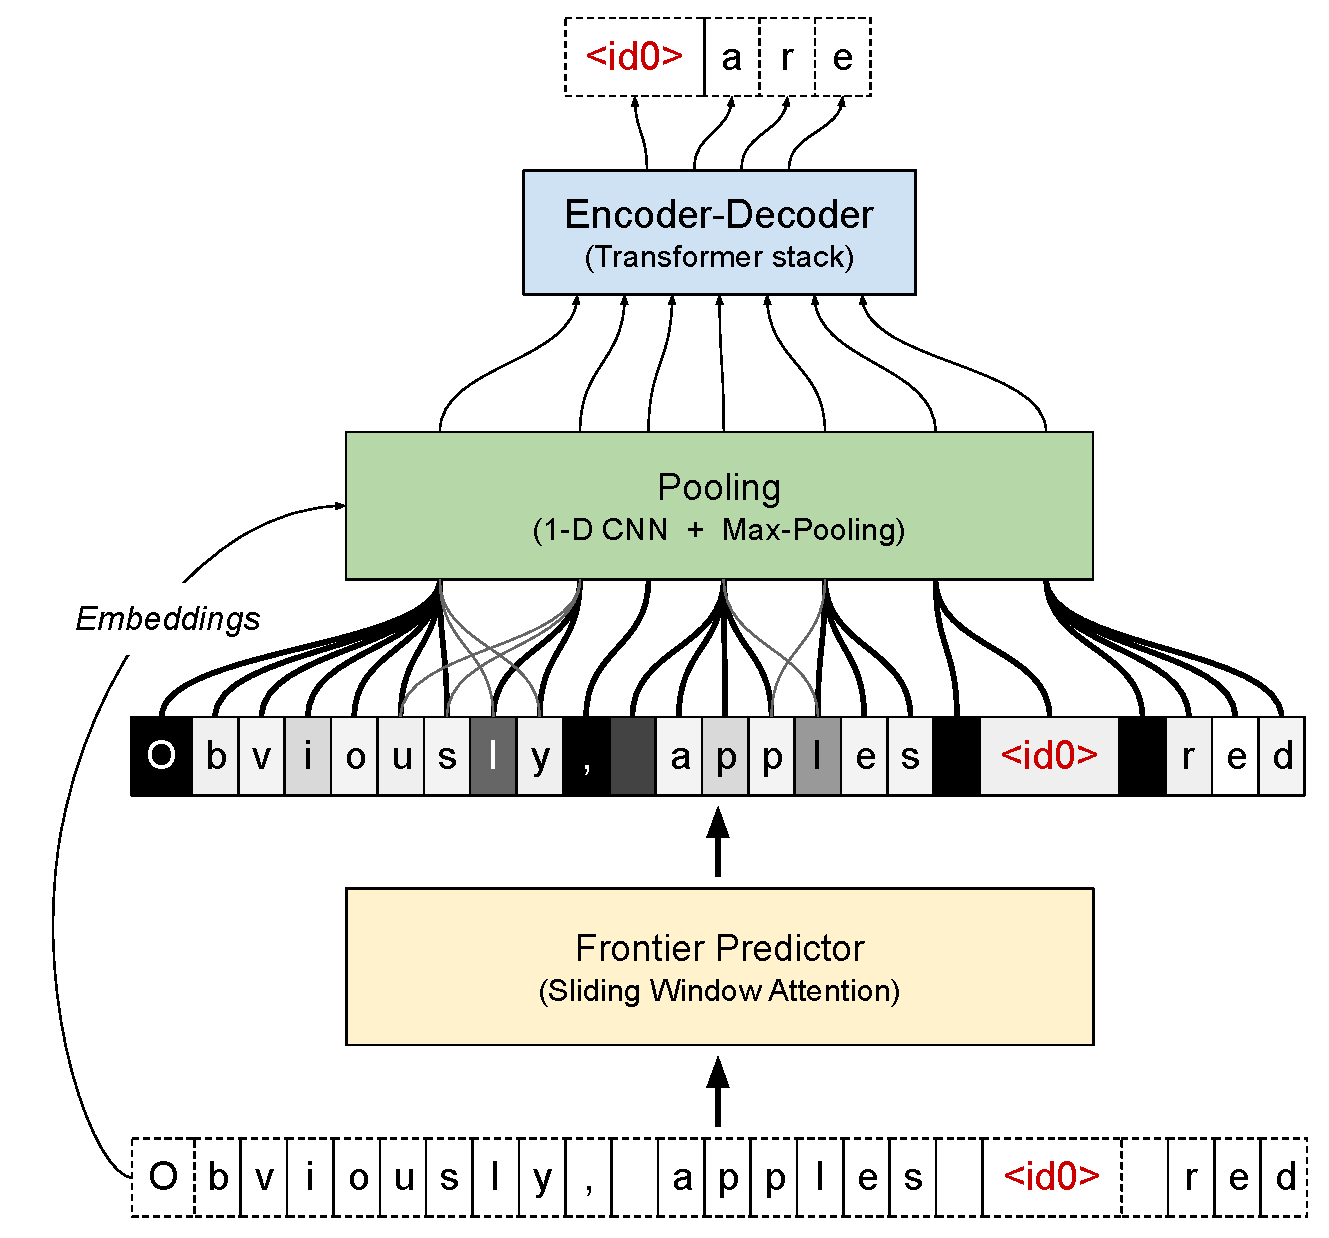
\includegraphics[width=0.6\linewidth]{sources/part_2/manta/images/full_difftok_schema.pdf}
    \caption{The differentiable tokenization scheme of MANTa-LM. Input bytes are first assigned a \textit{separation probability} using a Sliding Window Attention Transformer. These probabilities are used to compute the contribution of each byte embedding in the pooled representations of the \textit{blocks}. The block embeddings are fed to the Encoder-Decoder layers which predict the masked bytes. All the components are optimized with the LM objective.}
    \label{fig:overview_diagram}
\end{figure}

Hence, designing \textit{efficient} character-level models can be an interesting way forward to avoid phenomena such as the softmax bottleneck described in \Cref{chap:softmax_bottleneck}. In this chapter, we propose a gradient-based pooling module for language models based on character-level tokens, that reduces the overhead of processing longer sequences 

To overcome the inefficiency of character-level language modeling, \textit{tokenization-free} models \citep{clark2022canine,tay2021charformer} compress sequences using specialized modules that rely on a static segmentation strategy (see \Cref{sec:tokfree}).

We argue that learning a subword-level neural tokenization scheme together with input representations in an end-to-end fashion is beneficial for language modeling. In this work, we introduce MANTa, a gradient-based tokenizer and embedding module. It can easily be plugged-in to replace the classical combination of fixed tokenizers and trainable subword embedding matrices existing in most encoder-decoder models, without any increase in the total number of trainable parameters. We also introduce MANTa-LM, a Transformer encoder-decoder that incorporates MANTa and that is trained end-to-end. By learning a soft, adaptive segmentation of input sequences jointly with the LM pre-training objective, MANTa-LM produces byte-based representations with sequence lengths similar to those produced by static subword tokenizers. Additionally, by propagating gradients through our soft segmentation module during fine-tuning as well, we are able to adapt the segmentation to new domains, removing the limitations imposed by static subword tokenization.


    

Moreover, we show that MANTa-LM is robust to noisy text data and able to adapt to new domains while being significantly faster than byte-level models. Interestingly, MANTa learns a simple but explainable segmentation using only the LM objective while effectively reducing the length of byte sequences.

In summary, the contributions of this paper are the following: 
\begin{itemize}
    \item We introduce MANTa, a gradient-based tokenization and pooling module that can learn jointly with an encoder-decoder LM;
    \item We train MANTa-LM on English data and we evaluate its robustness to synthetic and natural variation and its ability to adapt to new domains compared to byte-level models.
    % \item We show that it performs similarly to token-level models on general-domain downstream tasks from the GLUE benchmark.
\end{itemize}


\section{MANTa}

% \begin{figure*}
% \centering
% \begin{subfigure}{.55\textwidth}
%   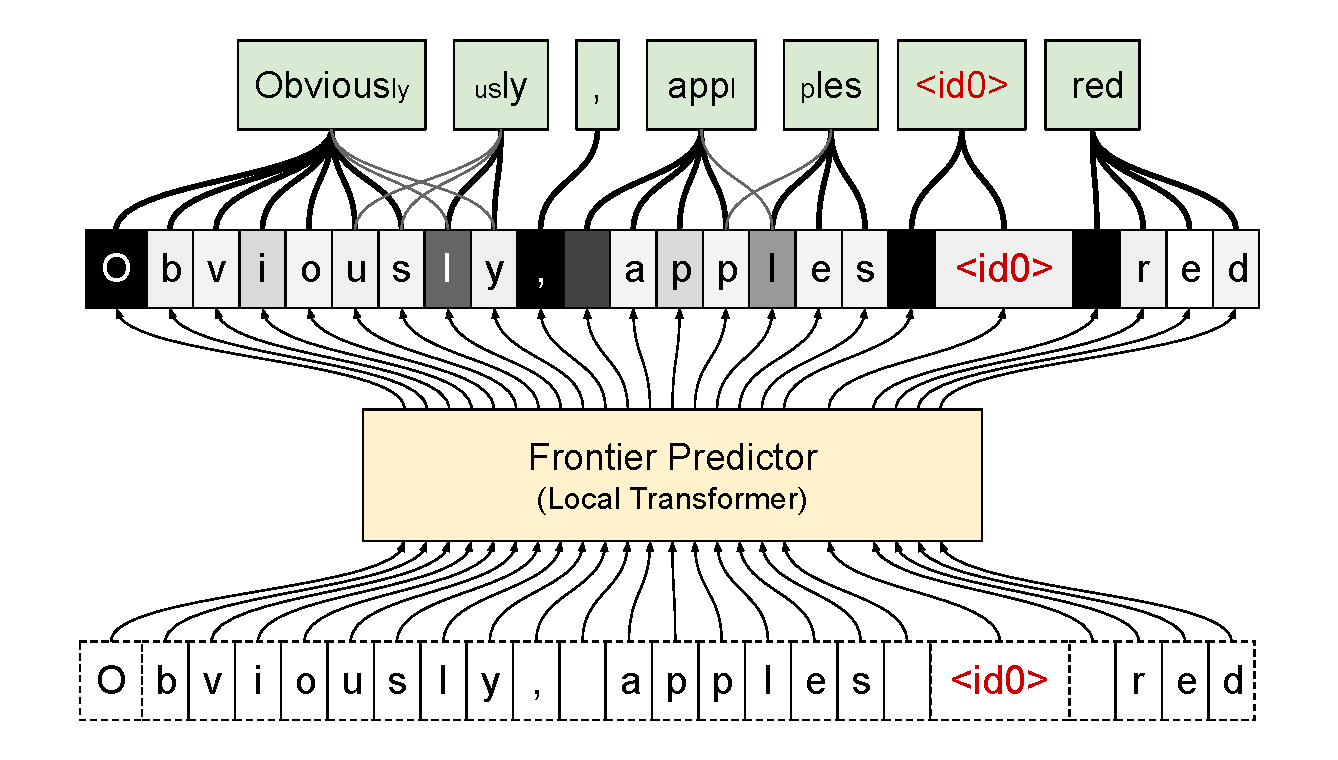
\includegraphics[width=\linewidth]{sources/part_2/manta/images/difftok_schema.pdf}
%   \caption{Our differentiable tokenization scheme.}
% \end{subfigure}
% \begin{subfigure}{.40\textwidth}
%   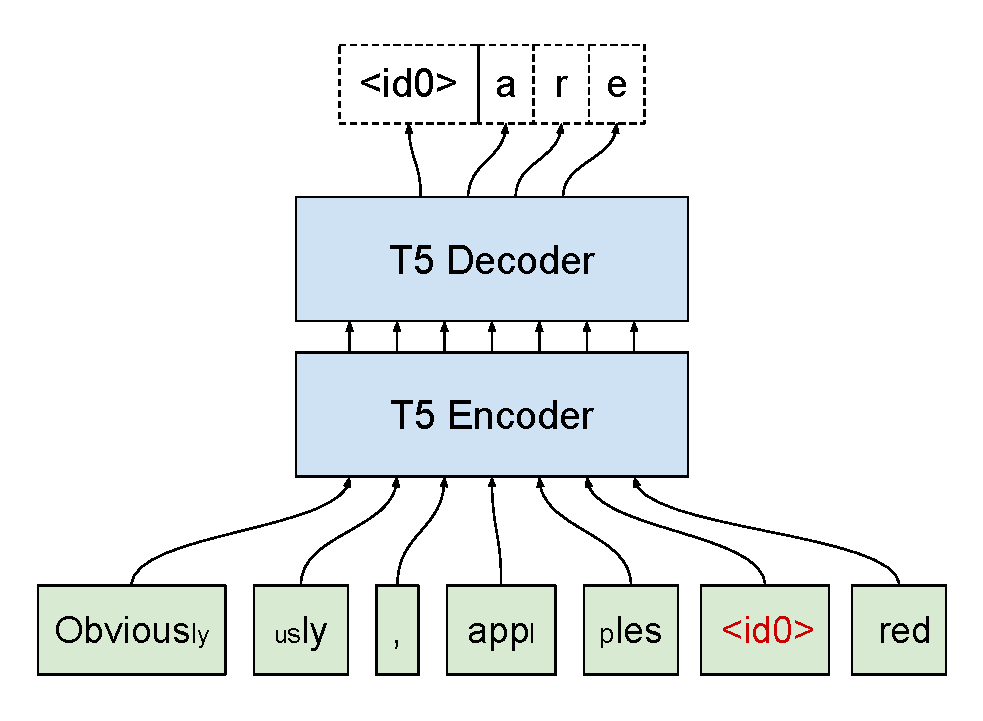
\includegraphics[width=\linewidth]{sources/part_2/manta/images/t5_schema.pdf}
%   \caption{This is a tiger.}
% \end{subfigure}
% \end{figure*}

\subsection{Differentiable Tokenization}
\label{sec:differentiable_tokenization}
Our main contribution is the introduction of an end-to-end differentiable tokenization architecture that consists in softly aggregating input bytes into what we refer to as \textit{blocks}. As an analogy with hard tokenization schemes, blocks can be compared to tokens with smooth borders.

We decompose the tokenization process into several differentiable operations, ensuring that our model can be trained end-to-end. Our approach consists in predicting a segmentation, and then combining byte embeddings according to this segmentation. MANTa can be divided in three different parts:
\begin{itemize}
    \item Predicting block frontiers using a parameterized layer to assign a probability $p_{F_i}$ to each input byte\footnote{Throughout this chapter, we use the notation $b_t$ instead of $w_t$ to improve clarity, as tokens do not correspond to word or subword level strings but rather to bytes.} $b_t$ of being a frontier;\footnote{$F$ in $p_{F_t}$ stands for \textit{Frontier}.}
    \item Building a byte-block unnormalized joint distribution using the frontier probabilities $(p_{F_t})_{t \in [1, L]}$ corresponding to a soft assignment from bytes to blocks;
    \item Pooling byte representations for each block $B_i$ weighted by the probability of each byte to belong in the current block $P(b_t \in B_i)$.
\end{itemize}

This process results in a sequence of embeddings that can be given directly to the encoder-decoder model. We provide an overview of the entire model in \Cref{fig:overview_diagram}, and we summarize the process of mapping byte embeddings to block embeddings in \Cref{sec:detailled_diagram}.

\begin{figure*}[!t]
    \centering\label{fig:detailled_diagram}
    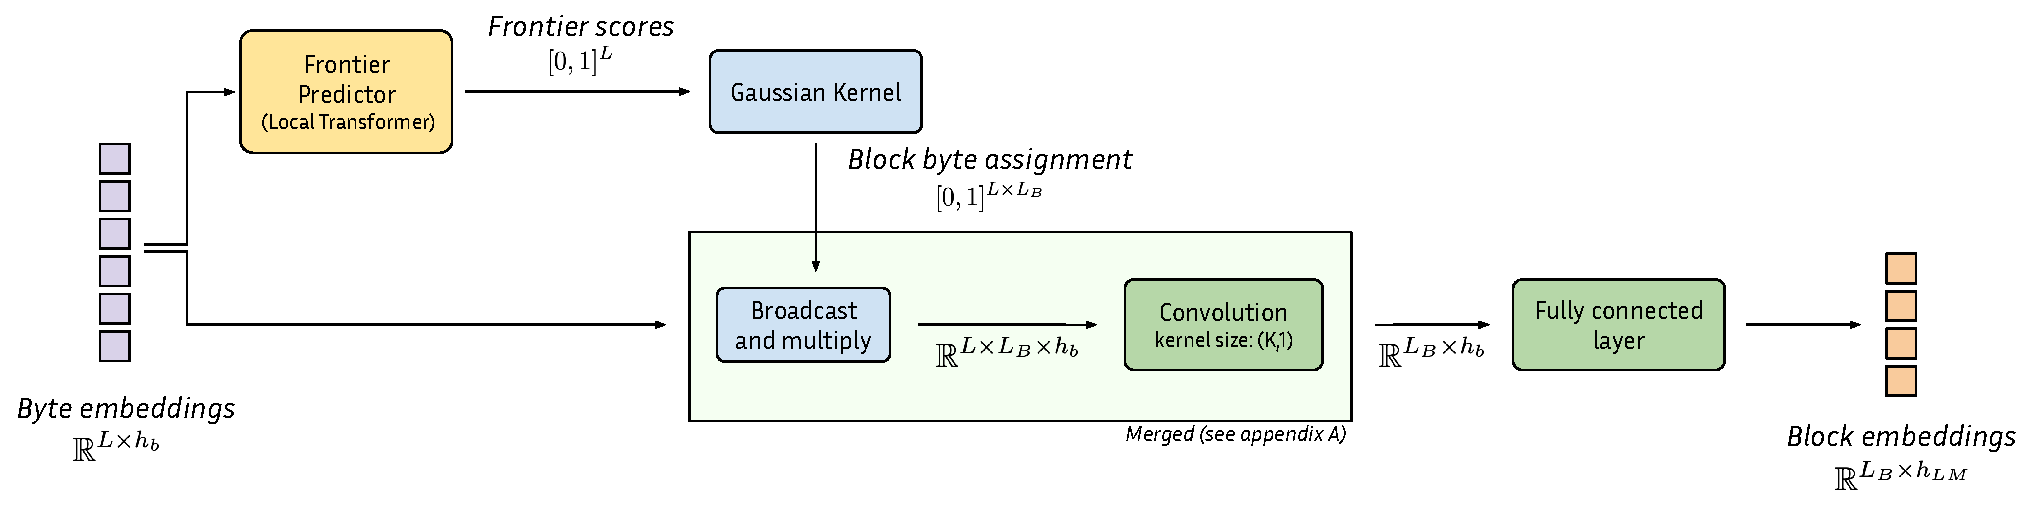
\includegraphics[width=0.9\linewidth]{sources/part_2/manta/images/MANTa_Tokenization_Module.pdf}
    \caption{A detailed view of the MANTa module. We denote by $h_b$ the dimension of the byte embeddings, by $h_{LM}$ the dimension of the block embeddings that will be fed to the encoder-decoder model, $L$ the length of the input sequence and $L_B$ the length of the block sequence. We omit batch sizes for simplicity.}
\end{figure*}

\subsection{Predicting Subword Frontiers}
\label{sec:frontpred}
% General principle: Seq2Seq model + sigmoid
% LSTM, local transformer
Our frontier predictor consists in a parameterized module mapping each byte $b_t$ to the probability of being a block frontier $p_{F_t}$. In a first part, we embed each byte $b_t$ to an embedding $e_{b_t}$. Working with bytes instead of characters allows modeling a larger array of symbols while having very small embedding matrices with $256\cdot d_m$ parameters, where $d_m$ is the hidden dimension of the model. Since the input sequences fed to the frontier predictor may be particularly long, we use a Transformer with sliding window attention~\citep{beltagy2020longformer}. This layer achieves a linear complexity with respect to sequence length by computing attention using only a local context. This reduced context forces the model to focus on local surface features rather than long-range dependencies which may be hard to model at the byte level.

We make the assumption that long-range dependencies are not relevant for segmentation and that this reduced context window should not harm the quality of the tokenization.


\subsection{Modeling the Byte-Block Assignment}
Once the frontier probabilities $(p_{F_t})_{t \in [1, L]}$ are predicted for the whole sequence, we use them to model an assignment between bytes and block slots. Each byte is given a probability distribution over the available block slots, and the expected block position of a byte in the block sequence increases along the byte sequence (i.e. the next byte is always more likely to be assigned to the next block).

Let us introduce $(B,\ b_t)$, the slot random variables for each byte $b_t$, describing the position of the block containing $b_t$ in the block sequence. In other words, the event $(B=i,\ b_t)$ describes the fact that the $t$-th byte belongs in the $i$-th block. These variables can only take values in $[1, L]$, as there cannot be more blocks than there are bytes. We can model the $(B,\ b_t)$ as a \textit{cumulative sum} of the random variables $F_t$: the position of the block in which a byte belongs is exactly the number of frontier bytes before this one.

Since $F_t \sim \mathcal{B}(p_{F_t})$, we can model the block index variables $B$ depending on the index of the bytes $b$ using the Poisson Binomial distribution $\mathcal{PB}$ which models the cumulative sum of Bernoulli variables: $\left(B,\ b_t\right) \sim \mathcal{PB}\left(\left(p_{F_k}\right)_{k \leq t}\right)$. There exists no closed form for this distribution's mass function, but some fast methods have been developed to avoid exploring the whole event tree \cite{BISCARRI201892, poibin_fft}. However, to reduce computational cost, we use a truncated Gaussian kernel $G$ with the same mean and variance to approximate the $(B,\ b_t)$ probability mass function:
$$
\forall i \in [1, L_B], P\left(B = i,\ b_t\right) \simeq P_{i,t} \triangleq \frac{1}{Z}G_{\mu_t, \sigma_t}(i)
$$
where $Z=\sum\limits_{1\leq i\leq L_B}G_{\mu_t, \sigma_t}(i)$ is a normalization term, and:
\begin{equation}
  \begin{cases}
    L_B = \min\left(L, \left(\mu_L + 3\sigma_L\right)\right)\\[11pt]
    \mu_t = \sum_{k=1}^{t} p_{F_k} \\[11pt]
    \sigma_t = \sqrt{\sum_{k=1}^{t} p_{F_k}\left(1-p_{F_k}\right)}
  \end{cases}
\end{equation}

We denote by $P_{i,t}$ the approximation of the probability of membership of the byte $t$ to block $i$. We display an example of this map at different steps during training in Figure~\ref{fig:mapping_example}. We truncate the block sequences after $(\mu_L + 3\sigma_L)$ since all the probabilities beyond this position are negligible.

\iffalse
\begin{figure*}
    \centering\small
    \begin{subfigure}[b]{0.45\textwidth}
    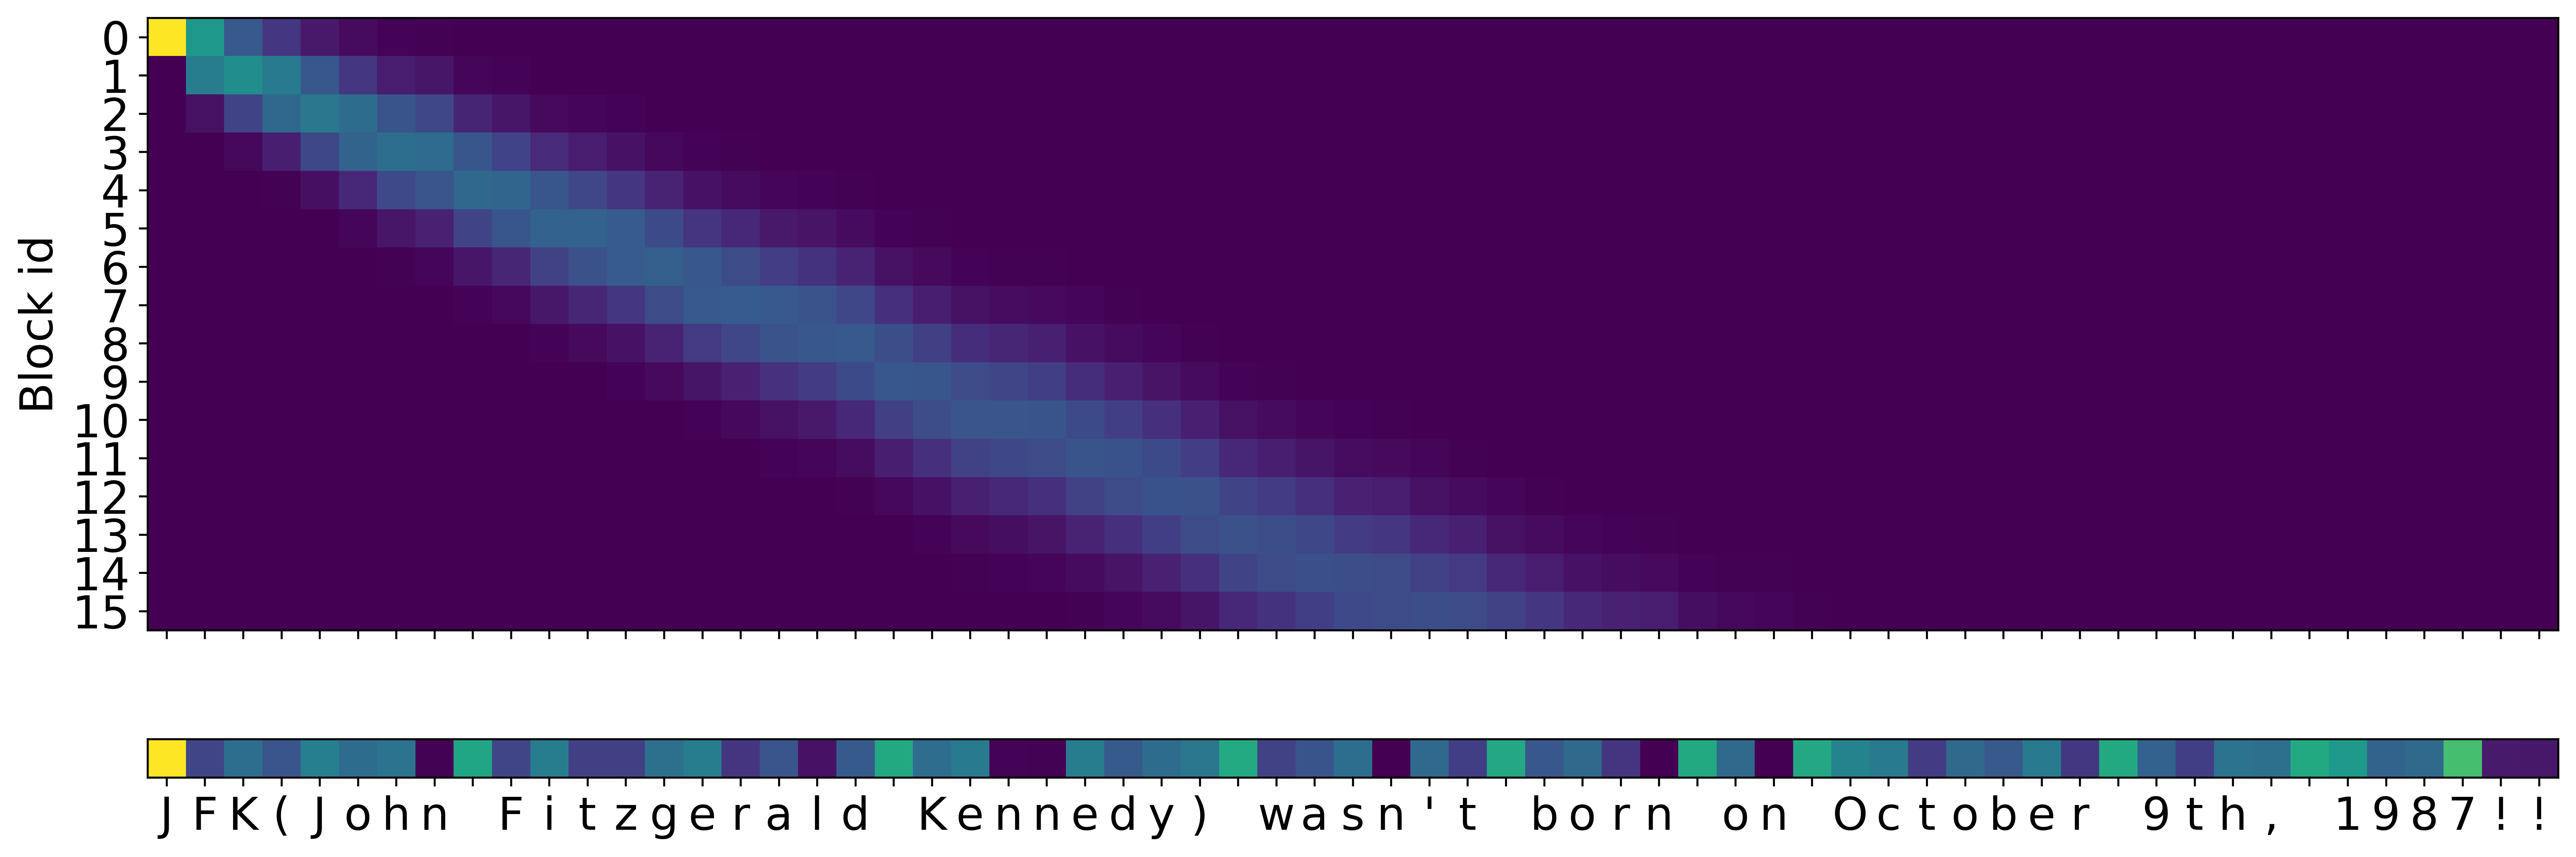
\includegraphics[width=\linewidth]{sources/part_2/manta/images/mapping_example_0.png}
    \caption{Step 0}
    \end{subfigure}\hfill
    \begin{subfigure}[b]{0.45\textwidth}
    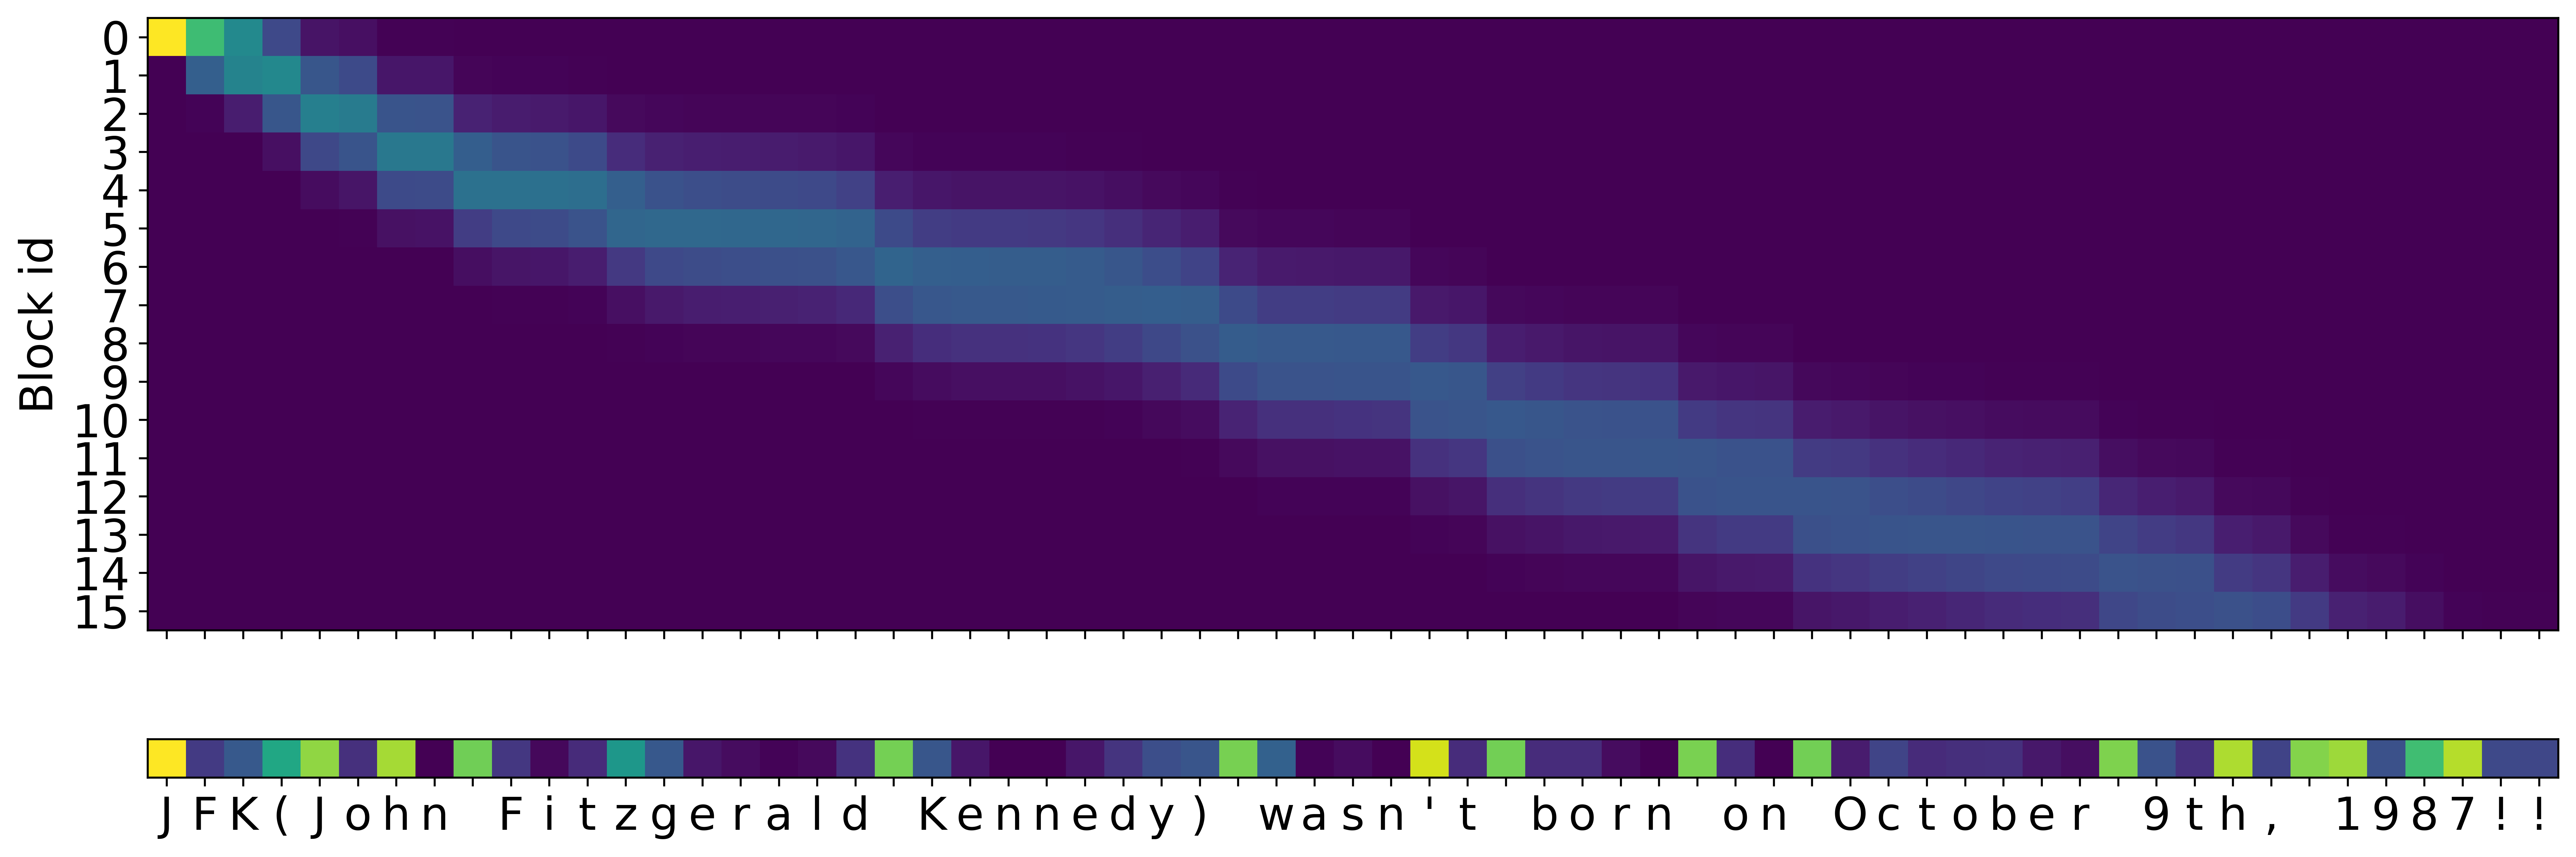
\includegraphics[width=\linewidth]{sources/part_2/manta/images/mapping_example_3000.png}
    \caption{Step 3,000}
    \end{subfigure}
    \begin{subfigure}[b]{0.45\textwidth}
    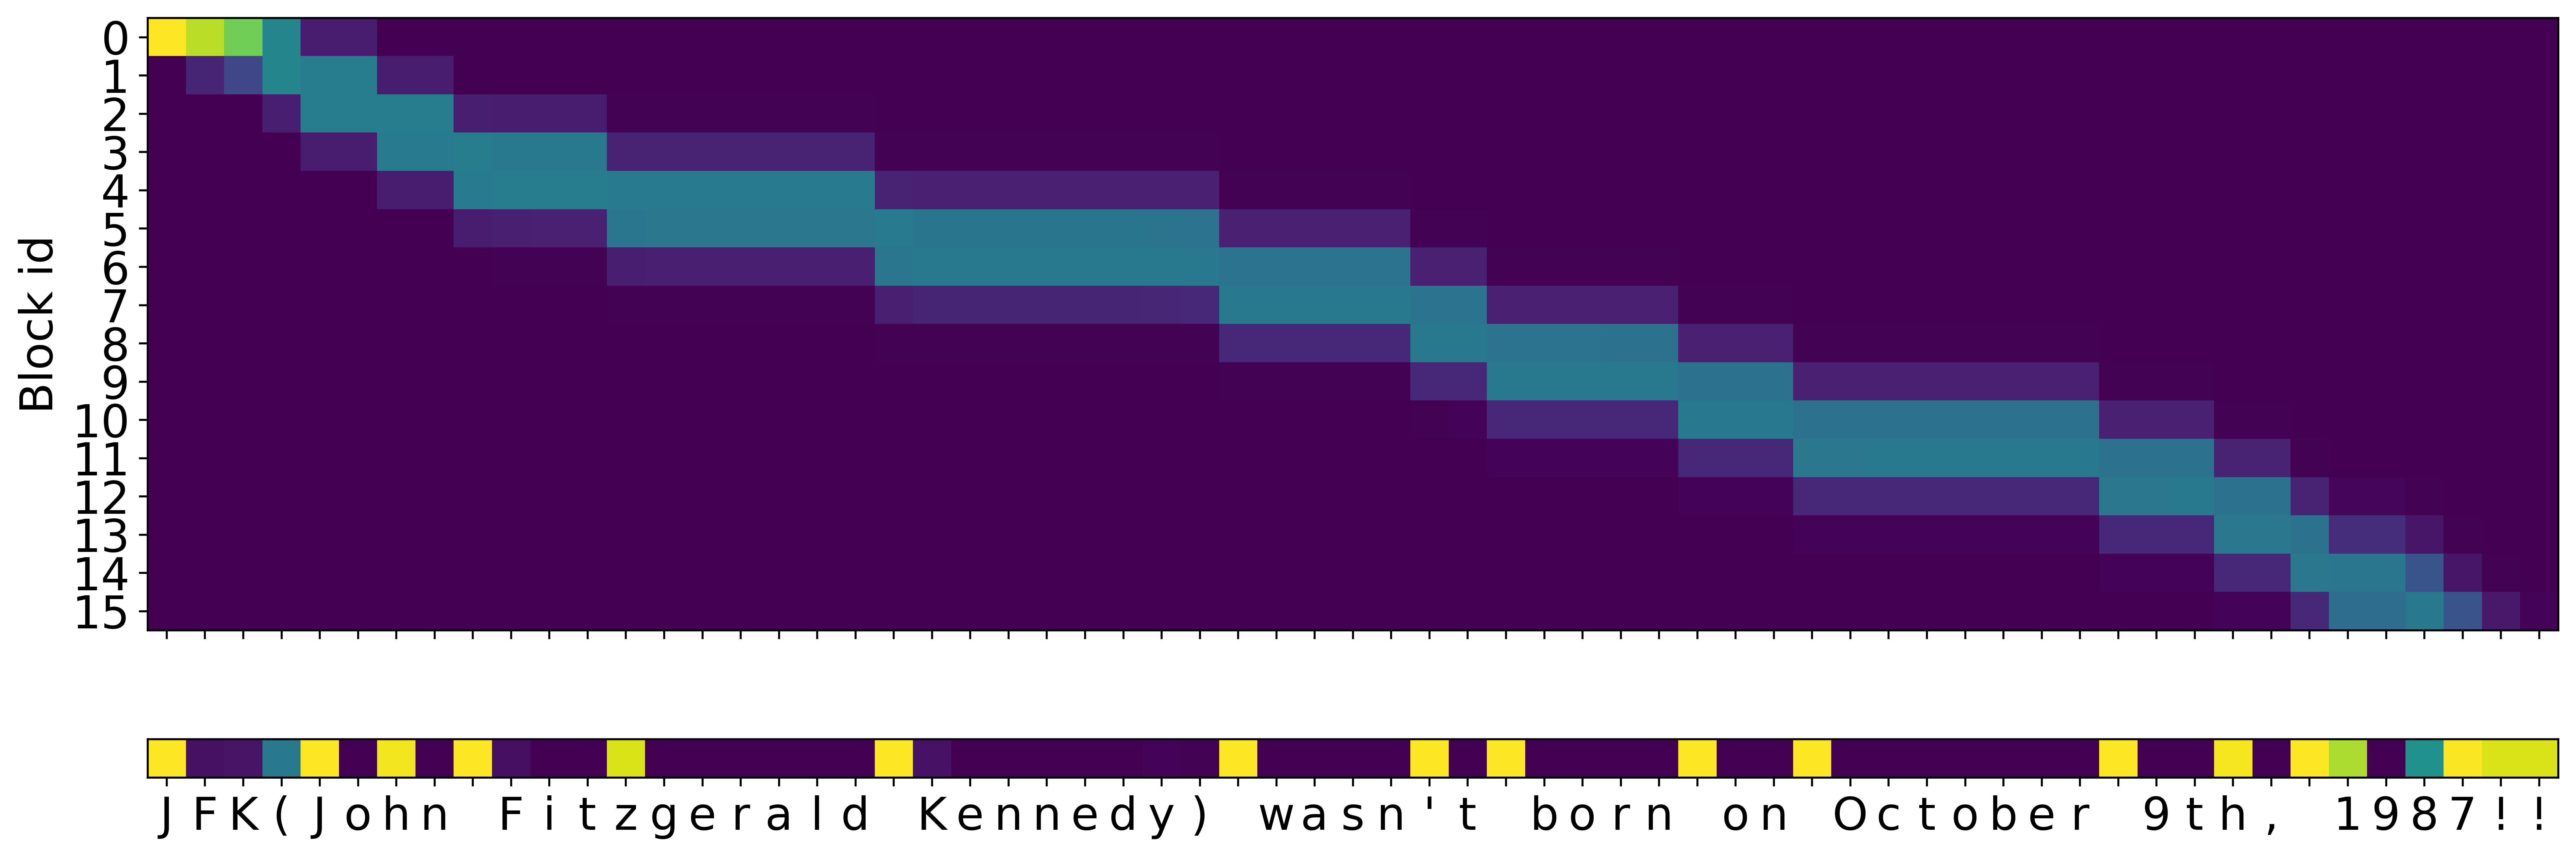
\includegraphics[width=\linewidth]{sources/part_2/manta/images/mapping_example_7000.png}
    \caption{Step 7,000}
    \end{subfigure}\hfill
    \begin{subfigure}[b]{0.45\textwidth}
    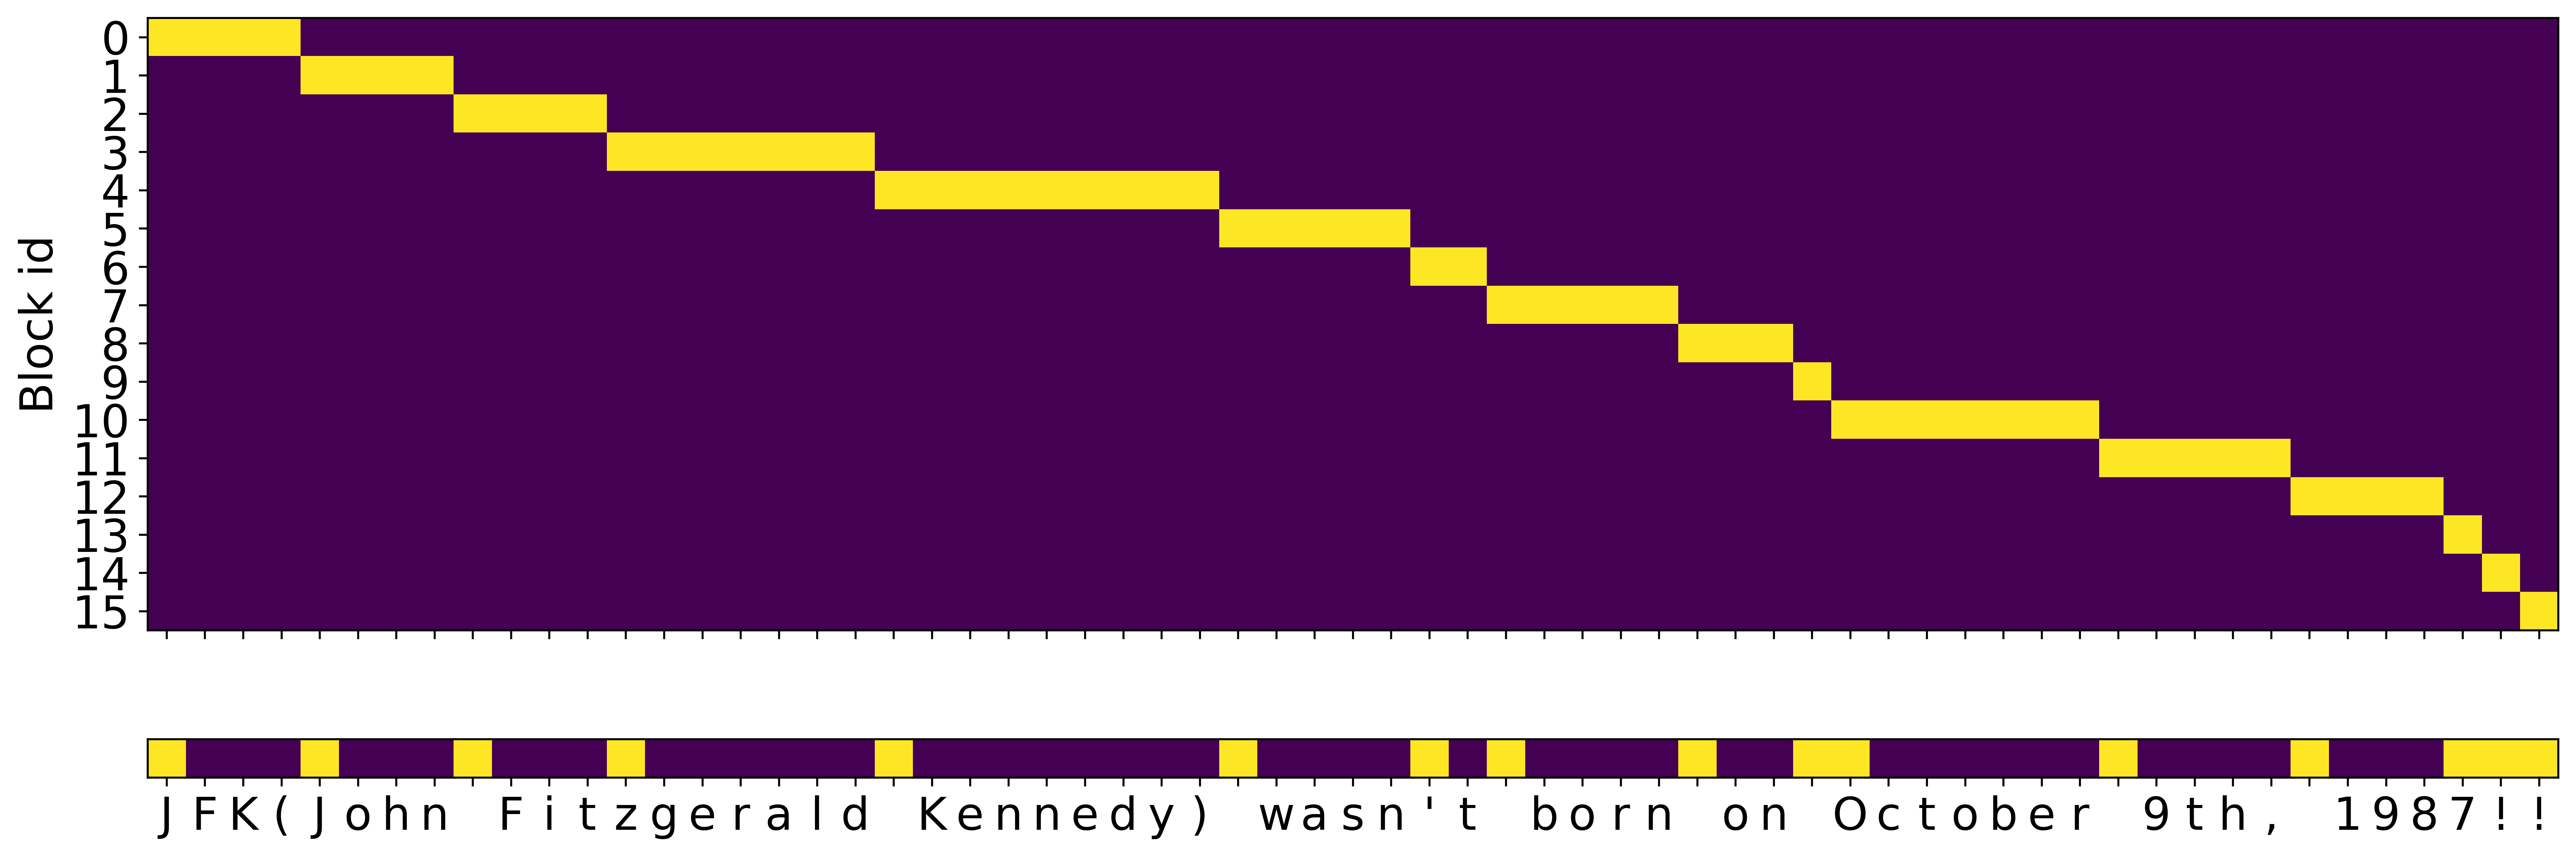
\includegraphics[width=\linewidth]{sources/part_2/manta/images/mapping_example_13000.png}
    \caption{Step 13,000}
    \end{subfigure}
    \caption{The block-byte soft assignment $P$ in the first pre-training steps. MANTa learns to downsample so that no information is lost through truncation, but also converges towards a sharp segmentation. }
    \label{fig:mapping_example}
\end{figure*}
\fi

\begin{figure}[ht!]
    \centering\small
    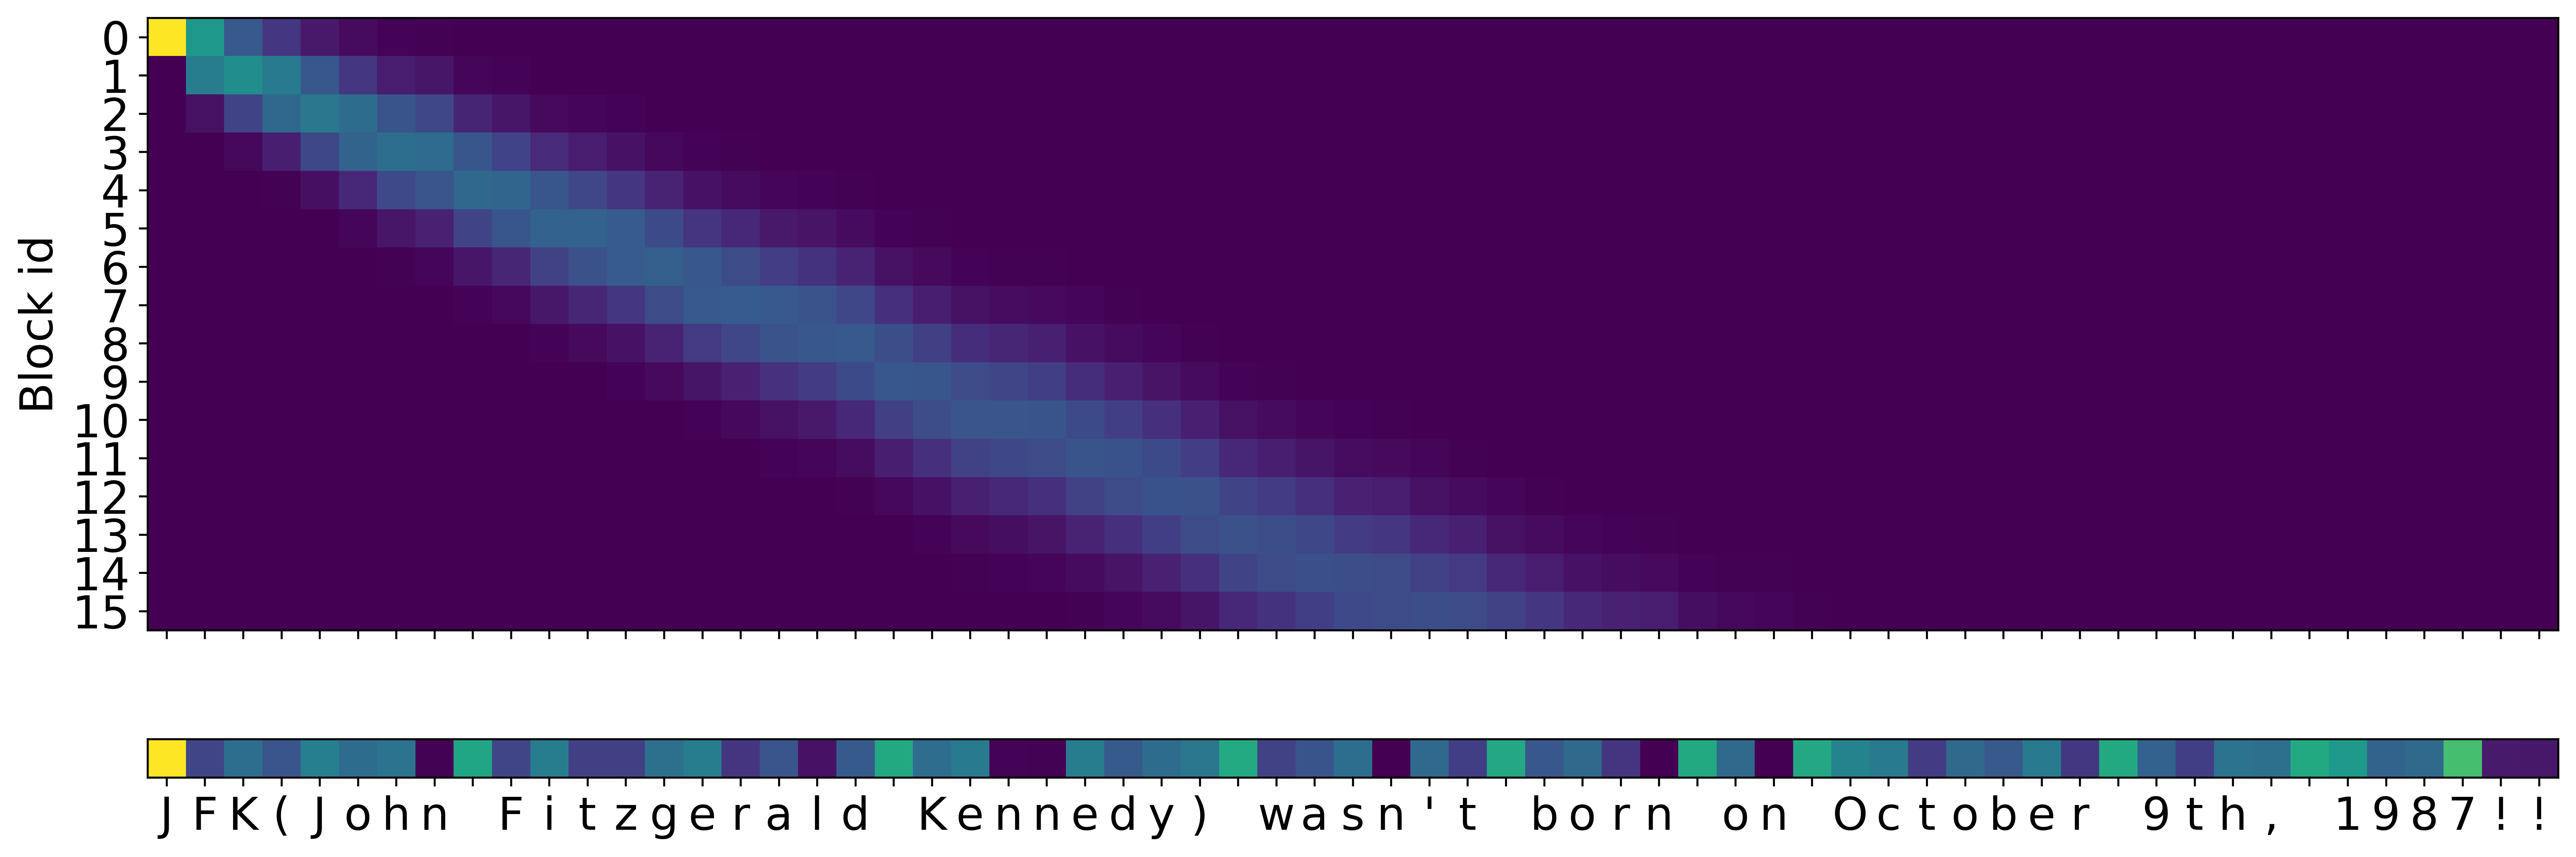
\includegraphics[width=0.6\columnwidth]{sources/part_2/manta/images/mapping_example_0.png}\\
    Step 0\\[2mm]
    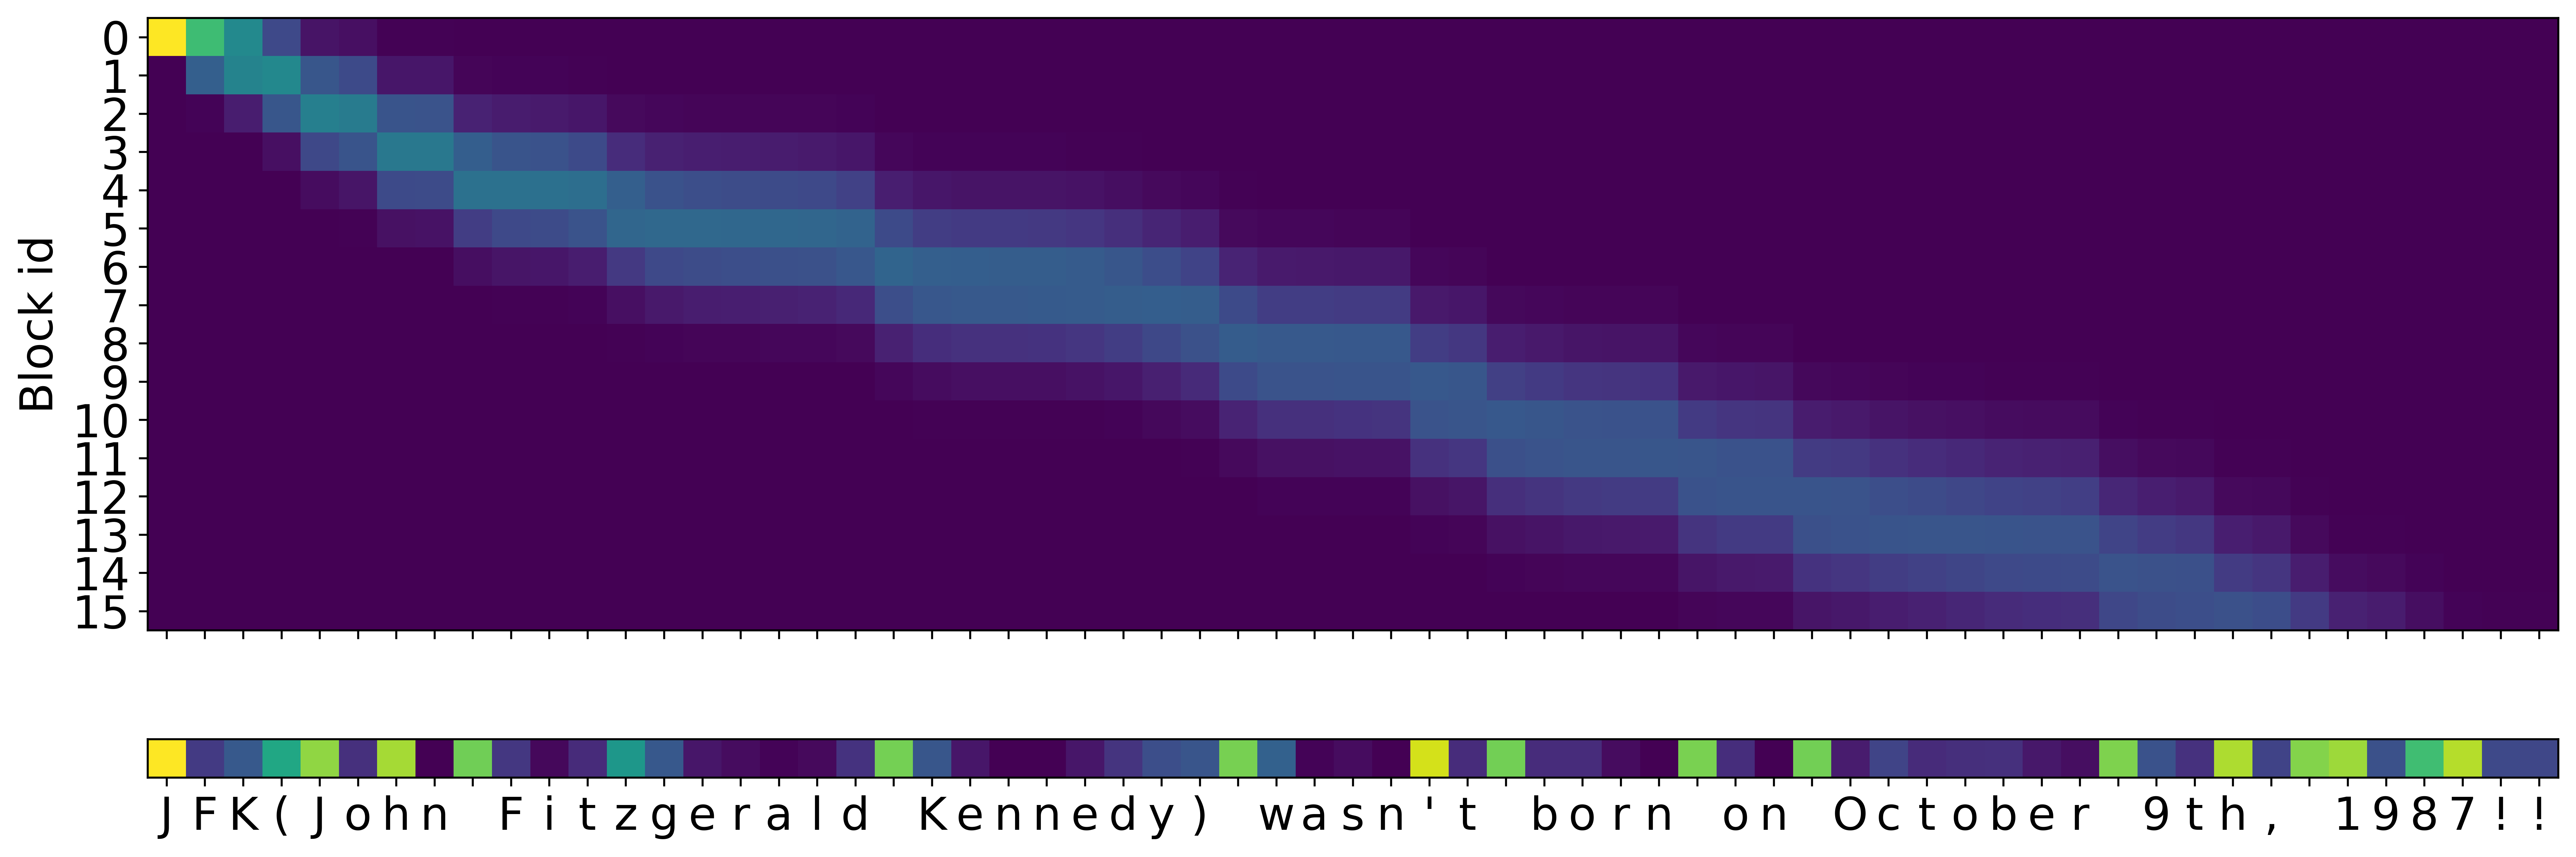
\includegraphics[width=0.6\columnwidth]{sources/part_2/manta/images/mapping_example_3000.png}\\
    Step 3,000\\[2mm]
    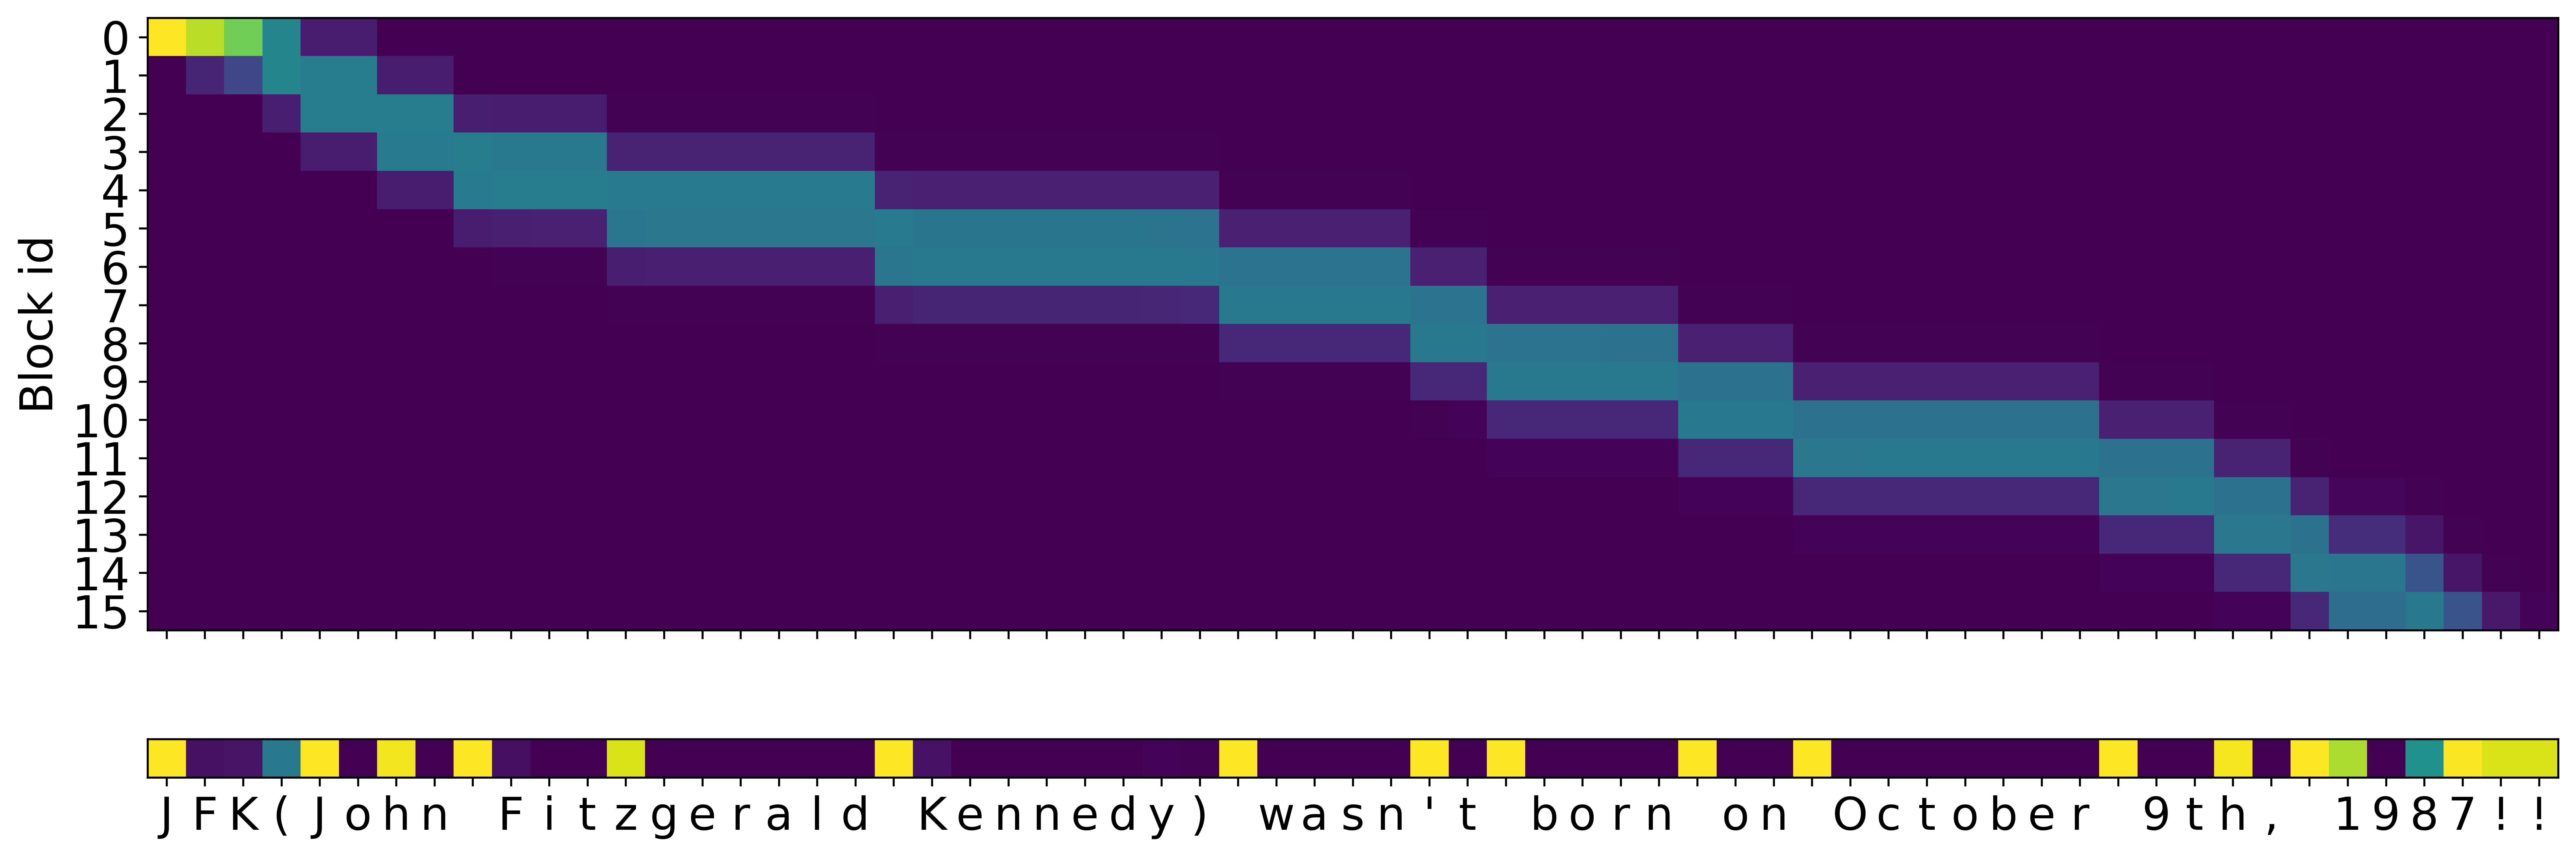
\includegraphics[width=0.6\columnwidth]{sources/part_2/manta/images/mapping_example_7000.png}\\
    Step 7,000\\[2mm]
    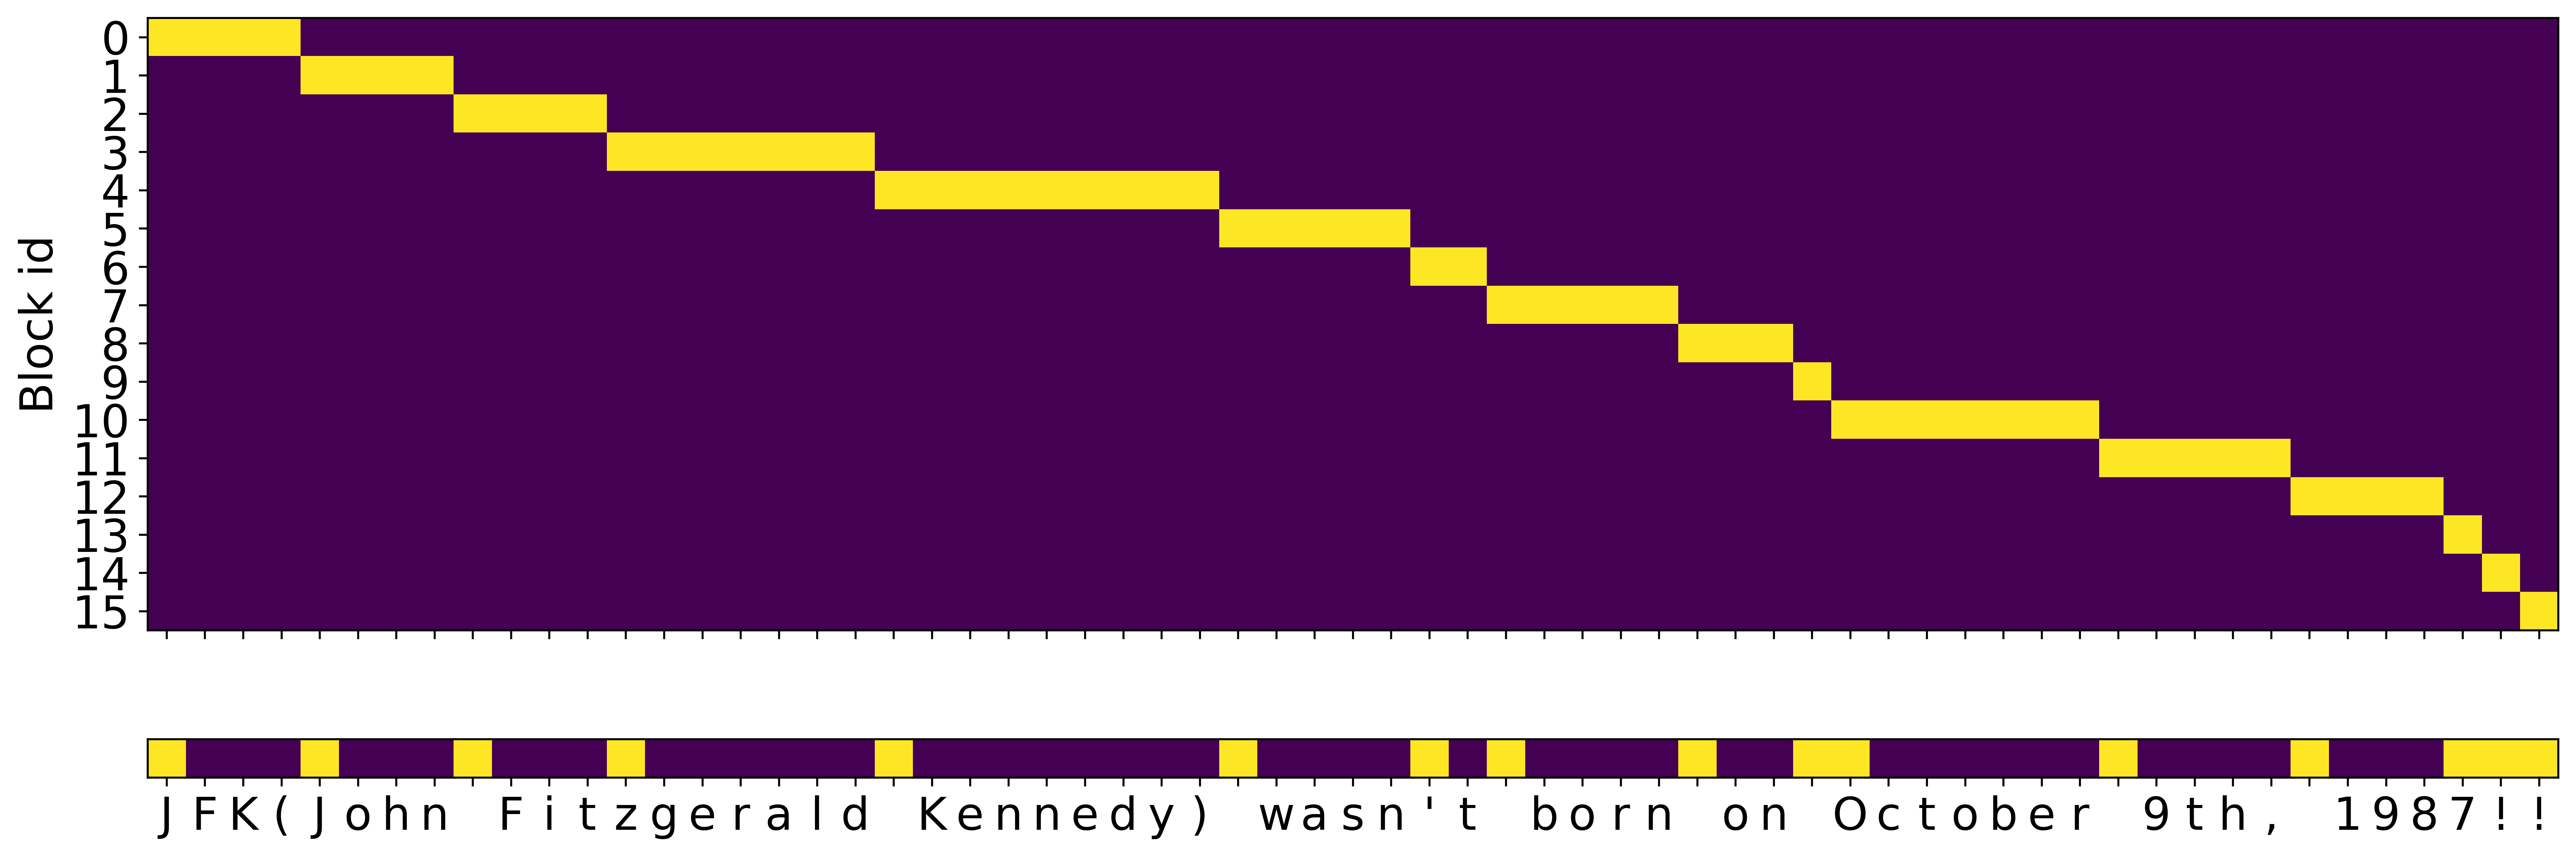
\includegraphics[width=0.6\columnwidth]{sources/part_2/manta/images/mapping_example_13000.png}\\
    Step 13,000\\
    \caption{The block-byte assignment $P$ during the first pre-training steps. MANTa learns to downsample input sequences so that no information is lost through truncation, but also converges towards a sharp segmentation.}
    \label{fig:mapping_example}
\end{figure}


\subsection{Pooling Block Embeddings}
\label{sec:pooling_block}
At this point in the forward pass, we have estimated the position of the block in which each input byte belongs, along with the block sequence maximum plausible length $L_B$.
%
In order to provide block embeddings to the LM, we now focus on the contribution of each byte to the block given by the block-byte assignment map. For each block position $i \in [1, L_B]$, this map actually provides an unnormalized contribution $(P_{i,t})_{t \in [1, L]}$ of each byte in this block. We can then use the byte embeddings $e_b$ from the frontier predictor described in \Cref{sec:frontpred} and, for the $i$-th block, build a block embedding where each byte $b_t$ contributes based on its probability of being in this block $P_{i,t}$.

To build $e^B_i$, the embedding of block $B_i$ in $i$-th position, we first compute the weighted byte embeddings ${\left(P_{i, t} \cdot e^b_t\right)_{t \in [1, L]}}\in \mathbb{R}^{d_b}$, with $d_b$ the hidden size of the byte embeddings. To make the block embeddings aware of the ordering of the bytes (e.g. so that \textit{ape} and \textit{pea} can have different representations), we proceed to a depthwise 1-D convolution along the dimension of the bytes after weighting. This convolution also improves the expressiveness of the block embeddings. 

Applying the 1-D convolution requires computing and storing $\mathcal{O}(L_B\times L\times d_b)$ parameters since we apply the 1D-convolution on every row of the weighted embedding map $P({e^b})^T$. Therefore, this operation may be particularly costly, especially if the frontier predictor outputs a high number of blocks. However, we can use the fact that the weighted embedding map has a special form to reduce the memory load when computing the convolution. Let $K$ be the convolution kernel size, $(C_j)_{j\in [1,K]}\in \mathbb{R}^{K\times d_b}$ the convolution filters and ``$\cdot$'' denote the element-wise product. Then, omitting padding and biases :
\begin{align*}
    e^B_i &= \max \limits_{t\in [1,L]} \sum \limits_{j=1}^{K} C_j \cdot \left( P_{i,t+j} \cdot e^b_{i+j} \right) \\
          &= \max \limits_{t\in [1,L]} \sum \limits_{j=1}^{K} P_{i,t+j} \cdot \left( C_j \cdot e^b_{t+j} \right)
\end{align*}

Notice how the product between the convolution filters and the byte embeddings $C_j \cdot e^b_{t+j}\in\mathbb{R}^{d_b}$ does not depend on the block anymore. We cache this computation, storing $\mathcal{O}(K\times L\times d_b)$ parameters and only later apply the convolution per block by summing these products with the block-byte membership map $P$. Caching greatly lowers the speed and memory requirements of MANTa, allowing to save $L_B-1$ element-wise products.\footnote{This caching would be exactly similar if the convolution was not depthwise.} $K$ is usually small, so the products can be stored easily.

We finally apply a max-pooling operation on the contextualized weighted byte embeddings for each block. This yields one embedding per block, with the same dimension as the byte embeddings. We use a linear layer to map the block embeddings to the right input dimension for the encoder-decoder model, i.e. its hidden size.


The final step consists in truncating the block embedding sequence to a fixed length $\hat{L} = \min(L_B, L / K)$ with $K\in \mathbb{N^*}$ a fixed \textit{truncation factor}. This simple heuristic ensures that all sequences fed to the encoder-decoder have a length at least $K$ times shorter than the input byte sequence length. We choose $K=4$ throughout the paper which is in average the number of bytes in an English BPE token. Most importantly, this truncation incentivizes the frontier predictor to produce sufficiently long blocks. We discuss the influence of this mechanism in more depth in \Cref{sec:truncation}.

% To obtain the final embedding sequence, we truncate aggressively the previously obtained sequence to a sequence 4 times shorter. This ensures that the encoder sequences have a similar length to subword sequences which limits the computational time. In addition, it incentivizes the frontier predictor to produce sufficiently long blocks. We discuss this mechanism in more depth in Section~\ref{sec:truncation}.

\subsection{Model Training}

%\subsubsection{Transformer stack}
We obtain from the differentiable tokenizer and pooling module a sequence of block embeddings that can be used exactly like subword embeddings. Thus, we use an encoder decoder architecture identical to T5 \citep{raffel2020t5}. Nevertheless, since we do not have a fixed subword vocabulary, our decoder operates at the byte level similarly to ByT5 \citep{xue2022byt5}.

% As we want our encoder-decoder model to behave similarly to the different T5 architectures, we truncate the block sequence to the appropriate sequence lengths (256 for the small architecture, and 512 for the base architecture). This also ensure that the block sequence length will not vary much during training which matters to the computation backbone (namely CudNN).

% We observed in our experiments that this truncation incited the tokenizer to avoid byte-level segmentation as it would imply losing information in the tokenization process.


\begin{table*}[]
\centering\small

\begin{adjustbox}{width=1\textwidth}

\begin{tabular}{cccccccccc}
\toprule
Model                                   & $|\theta|$ & MNLI      & QNLI & MRPC      & SST-2 & QQP       & STSB & COLA & AVG  \\ \midrule
$\text{T5}_{Small}$                     & 60M       & \textbf{79.7/79.7} & \textbf{85.7} & 80.2/86.2 & 89.0  & \textbf{90.2/86.6} & 80.0 & 30.3 & 76.6 \\[3pt]
$\text{MANTa-LM}_{Small}$ (ours)     & 57M          & 79.2/78.6 & 84.5 & \textbf{82.3/87.2}    & \textbf{89.6}  & 89.9/\textbf{86.5}    & \textbf{81.4} & \textbf{32.0} & \textbf{77.1} \\ \bottomrule
\end{tabular}
\end{adjustbox}
\caption{Results on dev sets for the GLUE benchmark for small models following our pre-training procedure.}
\label{tab:glue_small}


\end{table*}
% Please add the following required packages to your document preamble:
% \usepackage{booktabs}
\begin{table*}[t]
\centering\small
\begin{adjustbox}{width=1\textwidth}
\begin{tabular}{cccccccccc}
\toprule
Model                                   & $|\theta|$ & MNLI      & QNLI & MRPC      & SST-2 & QQP       & STSB & COLA & AVG  \\ \midrule
$\text{BERT}_{Base}^\dagger$            & 110M       & \textbf{84.4} / -  & 88.4 & 86.7/-    & \textbf{92.7}  & -         & -    & -    & -    \\[3pt]
$\text{T5}_{Base}^\dagger$              & 220M       & 84.2/\textbf{84.6} & 90.5 & \textbf{88.9/92.1} & \textbf{92.7} & \textbf{91.6/88.7} & \textbf{88.0} & 53.8 & 84.3 \\ \midrule
$\text{CharBERT}_{Base}^\mathsection$   & 125M       & -         & \textbf{91.7} & 87.8/-    & -     & 91/-      & -    & \textbf{59.1} & -    \\[3pt]
$\text{Byte-level T5}_{Base}^\dagger$   & 200M       & 82.5/82.7 & 88.7 & 87.3/91.0 & 91.6  & 90.9/87.7 & 84.3 & 45.1 & 81.5 \\[3pt]
$\text{Charformer}_{Base}^\dagger$      & 203M       & 82.6/82.7 & 89.0 & 87.3/91.1 & 91.6  & 91.2/88.1 & 85.3 & 42.6 & 81.4 \\[3pt]
% $\text{MANTa-LM}_{Base}$ (ours)          & 200M       &    80.6/81.0       &  85.3    &    83.4/88.2       &   92.0    &       82.2/85.4    &   76.6   &   37.0   &   77.3   \\ [3pt] \bottomrule
% $\text{MANTa-LM}_{Base}$ (ours)     & 200M        & 78.1/78.2 & 88.6 & 83.6/88.6 & 91.0 & 70.7/88.6 & 74.1 & 45.0 & 78.7  \\ [3pt] \bottomrule
$\text{MANTa-LM}_{Base}$ (ours)     & 200M        & 77.5/78.8 & 88.2 & 82.4/88.2 & 91.3  & 90.8/87.7 & 79.2 & 51.0 & 80.3\\ [3pt] \bottomrule
\end{tabular}
\end{adjustbox}

\caption{Results on dev sets for the GLUE benchmark. $\dagger$ indicates results obtained by \citet{tay2021charformer}, which are very similar to our models in terms of compute, but use a smaller batch size which may enhance their performance. $\mathsection$ indicates results obtained by \citet{ma-etal-2020-charbert}. The top section concerns model trained using a subword tokenizer.}
\label{tab:glue}
\end{table*}

\subsection{Pre-Training Details}

\paragraph{Objective}
Our objective is identical to the one used in ByT5. We mask 15\% of bytes randomly and choose a number of spans such that each has an average length of 20 bytes. Each span is then replaced by an \texttt{<extra\_id\_i>} token with \texttt{i} identifying the order of the span in the sequence. On the decoder side, the model has to predict in an autoregressive way the span identifier and the masked bytes.

\paragraph{Data}
We pre-train our model on English text data using C4 \citep{raffel2020t5}, a large corpus scraped from the Internet. This corpus is particularly suited to our pre-training due to its diversity in terms of content and linguistic variations. In addition, it enables a better comparison with other tokenizer-free models trained using it such as Charformer. Since this dataset is not available publicly, we use the English split of the mC4 distributed by AllenAI. We filter long documents containing more than $2^{15}$ bytes, which is a simple proxy to remove important quantities of unwanted code data.

\paragraph{Hyperparameters}
We pre-train two versions of our model: $\text{MANTa-LM}_{Small}$ and \\
$\text{MANTa-LM}_{Base}$. Each of them stacks a $\text{MANTa}_{Small}$ (resp. $\text{MANTa}_{Base}$) tokenizer and embedding module and a $\text{T5}_{Small}$ (resp. $\text{T5}_{Base}$) encoder-decoder model stripped of its tokenizer and subword embedding matrix. Details about $\text{MANTa}$ hyperparameters can be found in \Cref{sec:appendix_hp}.

Following T5 and ByT5, we use the Adafactor optimizer with a learning rate of $10^{-2}$ for the encoder-decoder model, parameter scaling for the whole system and no weight decay. However, to maintain stability of our differentiable tokenizer, we use a learning rate of $10^{-3}$ for the parameters of the byte embeddings, the frontier predictor, and the pooling module. We also use a triangular learning rate schedule with 1000 (resp. 5000) warm-up steps for batch size 1024 (resp. 64).

\paragraph{Training} We train $\text{T5}_{Small}$, $\text{MANTa-LM}_{Small}$, and $\text{MANTa-LM}_{Base}$ for 65k steps with a batch size of 1024. Sequence lengths are respectively 1024 for $Small$ models and 2048 for the $Base$ model. Thus, the models are trained on roughly the same amount of bytes as in \citet{tay2021charformer}, where a batch size of 64 is used for 1M steps. 

We also train a $\text{ByT5}_{Small}$ model on the same data, using a batch size of 64 and a sequence length of 1024. We consider the ``Scaled'' architecture which provides the encoder with more layers than the decoder \cite{xue2022byt5}. To avoid prohibitive computation costs and ensure fairness in terms of available resources between models, we limit its training time to the one of $\text{MANTa-LM}_{Small}$. Hence, our $\text{ByT5}_{Small}$ is only trained for 200k steps.



\section{Experiments and Results}
\subsection{Evaluation on GLUE}

To ensure that our model is competitive with existing language models exploiting subword tokenization algorithms, we evaluate it on several English datasets and compare it with other baseline models.

\paragraph{Setup} We use GLUE~\cite{wang-etal-2018-glue}, a Natural Language Understanding benchmark consisting of 7 tasks, to evaluate our model. Similarly to T5, we cast the classification tasks as generation tasks where the model has to predict autoregressively the bytes forming the answer. 

We compare our model to an encoder-decoder model with subword tokenization (pre-trained with the same denoising objective as T5) and a fully byte-level encoder-decoder, similar to ByT5. We compare $Small$ models with our pre-trained versions, and $Base$ models with results mentioned in \citet{tay2021charformer}. We report the number of parameters given in \citet{tay2021charformer} for $\text{Byte-level T5}_{Base}$, and gather from its low value that their implementation corresponds to a $\text{T5}_{Base}$ architecture trained on byte-level inputs. 

\paragraph{Results} Results can be found on Tables~\ref{tab:glue_small} and~\ref{tab:glue}. Overall, MANTa-LM exhibits a performance slightly below Charformer but stays within a small margin on average (1.1 points below). Nonetheless, the main objective of our method is to balance decent performance with robustness and speed which we show in the following sections.

% We are on par with other state-of-the-art models, albeit somewhat below on a number of tasks and above on SST-2, thus showing that our approach does not have a significant (negative) impact on standard, in-domain scenarios. \footnote{The gap between models we pre-trained (ByT5 and MANTa-LM) and the literature may indicate that our results could be improved by longer training. We will investigate this in the coming weeks and incorporate the results in the final version of the paper, should the paper be accepted. However, our main objective is not to improve the state of the art for in-domain settings, but to show how our approach can improve out-of-domain and noisy settings, which is the focus of the next Section.}


\subsection{Robustness to Domain Change}
Static subword tokenizers tend to show important limitations when used with texts originating from a domain unseen during training. For instance, \citet{el-boukkouri-etal-2020-characterbert} show that tokenizing medical texts with a tokenizer trained on Wikipedia data often results in an over-segmentation of technical terms which in turn affects the downstream performance. By removing this static bottleneck in MANTa-LM, we hope that it should be able to adapt more easily to new domains. To test this hypothesis, we finetune it on a medical Natural Language Inference dataset.

\begin{table}[t]
\centering\small
\begin{tabular}{lc}
\toprule
Model                                   & Accuracy  \\ \midrule
$\text{BERT}_{Base}^\ddagger$           & 77.7      \\
$\text{CharacterBERT}_{Base}^\ddagger$  & 77.9      \\
$\text{T5}_{Small}$                     & 75.3      \\ 
$\text{MANTa-LM}_{Small}$ (ours)     & 75.6      \\\bottomrule
\end{tabular}
\caption{Results on MedNLI. $\ddagger$ indicates results from \citet{el-boukkouri-etal-2020-characterbert}, who use a different pre-training corpus than C4. All other results are from models trained with our codebase.}
\label{tab:mednli}
\end{table}

\paragraph{Setup} We finetune MANTa-LM on \textsc{MedNLI} \citep{romanov-shivade-2018-lessons}, a dataset consisting of 14,049 sentence pairs extracted from clinical notes. We follow the same finetuning setup than for the GLUE Benchmark i.e. use the same batch size and learning rate. We compare our results to the ones obtained by \citet{el-boukkouri-etal-2020-characterbert} with models pretrained on the general domain.

\paragraph{Results} We present our results on \Cref{tab:mednli}. Although we notice a significant drop in performance compared to the encoder models trained by \citet{el-boukkouri-etal-2020-characterbert}, we believe this drop may be due to the different pretraining data used---CharacterBERT uses splits of Wikipedia, which may be helpful to learn some technical terms related to the clinical domain---, and the different model sizes---CharacterBERT uses all of its parameters to encode example, while we keep half of the parameters in the decoder. Nonetheless, we note that MANTa-LM reaches a better performance than its subword tokenization counterpart T5.

\subsection{Robustness to Noisy Data}
Although LMs may learn complex patterns even from noisy input texts, this ability is conditioned by how the tokenizer segments character sequences. Since MANTa is not static and can be finetuned on non-standard data, we expect it should be able to learn to be more robust to variation/noise compared to a subword tokenizer paired with a LM. To evaluate this hypothesis, we study how MANTa-LM behaves on both naturally occurring text variation and multiple levels of synthetic noise.

\subsection{Naturally Occurring Noise}
\paragraph{Setup} Similarly to \citet{tay2021charformer}, we test our model on a toxicity detection task constructed with user generated data. We use the \textsc{ToxicComments}\iffalse\footnote{Other names for this dataset include ``Jigsaw Toxicity Prediction'' and ``Wiki Toxicity.''}\fi{} dataset \citep{wulczyn2017ex} which contains 223,549 sentences annotated with a binary label indicating whether each sentence can be classified as toxic or not. We also use the same finetuning setup here as the one used for evaluating on the GLUE benchmark. 

\paragraph{Results} We present our results in \Cref{tab:toxic} and compare them to the ones reported in \citet{tay2021charformer}. As expected, noisy user generated data is particularly harmful for models using subword tokenization. On the other hand, constructing sentence representations with byte-level information  helps and our model is more accurate than Charformer. This gain may be due to a better segmentation of specific terms encountered in the data.


\begin{table}[t]
    \centering\small
    \begin{tabular}{lc}
    \toprule
    Model                                   & Accuracy      \\ \midrule
    $\text{T5}_{Base}^\dagger$              & 91.5          \\
    $\text{Charformer}_{Base}^\dagger$      & 92.7          \\
    $\text{MANTa-LM}_{Base}$ (ours)      & {\textbf{93.2}}   \\\bottomrule
    \end{tabular}
    \caption{Results on the \textsc{ToxicComments} dataset. Results indicated by $\dagger$ are from~\citet{tay2021charformer}.}
    \label{tab:toxic}
    \end{table}


\subsection{Synthetic Noise}
\paragraph{Setup} We also compare T5 and ByT5 with our approach when facing different levels of noise. This study pictures how these models react to unseen noise at evaluation time (\textsc{Dev-Only} setup) and how they adapt to a given noise via fine-tuning (\textsc{Train-Dev} setup). We apply synthetic noise at different levels $\tau\in\{0.05, 0.10, 0.15\}$ by picking randomly $\tau \times L$ positions in the byte sequences and equiprobably deleting, replacing or inserting bytes at these positions.



\begin{figure}[t]
    \centering
    \begin{subfigure}[b]{0.48\columnwidth}
         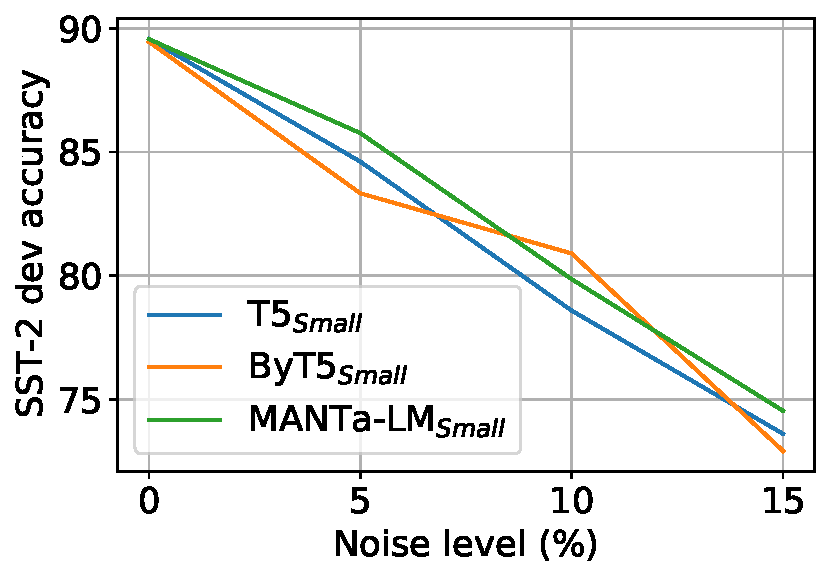
\includegraphics[width=\linewidth]{sources/part_2/manta/images/noise_curve_dev.pdf}
         \caption{\textsc{Dev-Only}}
    \end{subfigure}
    \begin{subfigure}[b]{0.48\columnwidth}
         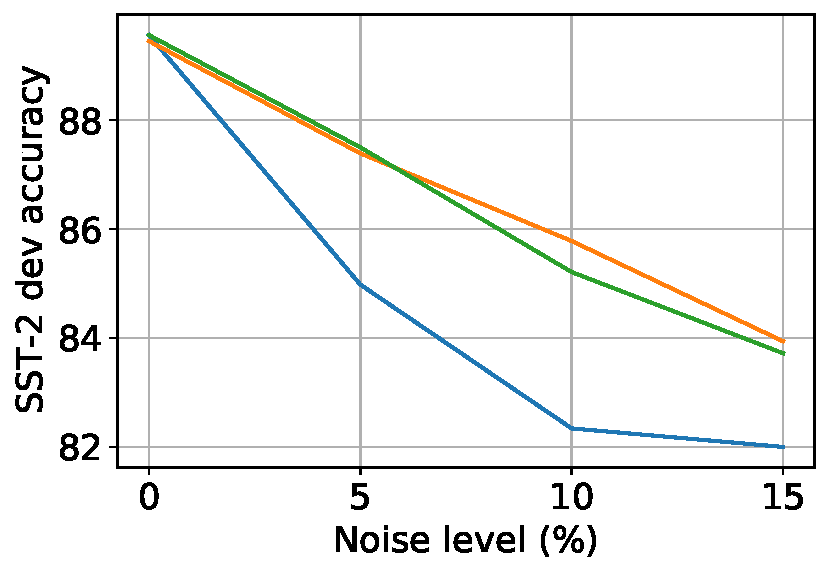
\includegraphics[width=\linewidth]{sources/part_2/manta/images/noise_curve.pdf}
         \caption{\textsc{Train-Dev}}
    \end{subfigure}
    \caption{Best accuracy on the SST-2 development set as the noise level increases. The \textsc{Train-Dev} setting corresponds to models finetuned on noisy data while models in the \textsc{Dev-Only} setting have been finetuned on clean data.}
    \label{fig:noisy_sst2}
\end{figure}

% Par contre, il serait bien de modifier légérement ces figures:
% - mettre la légende dans les 2 ou dans celle du haut, pas dans celle du bas (bien sûr vous aviez fait ça à juste titre dans la configuration précédente)
% - faire en sorte que les sous-titres (a) et (b) soient plus proches de la figure qu'ils légendent et que le (a) soit moins proche de la figure du dessous
% Ecrivez qqch si vous avez vu ces lignes :)

\paragraph{Results} The results can be found in \Cref{fig:noisy_sst2}. We found that models performed similarly for the different noise levels in the \textsc{Dev-Only} setting. On the contrary, in the \textsc{Train-Dev} setting, MANTa-LM can be finetuned as well as ByT5 for all levels of noise, while the performance of T5 quickly degrades.

\section{Training Speedups}

In terms of speed, we compare our model to $\text{MANTa-LM}_{Small}$ to $\text{T5}_{Small}$ counterparts: one that is trained at the classical subword-level, and one trained at byte-level, hence using sequences that are roughly 4 times longer. We also report the speed of the larger $\text{ByT5}_{Small}$ architecture as described in \citet{xue2022byt5}. The results are presented in \Cref{tab:speed}.

MANTa-LM is approximately 4 times faster than $\text{Byte-level T5}_{Small}$, and 5 times faster than $\text{ByT5}_{Small}$, which can be explained by the reduced sequence length we use in the encoder-decoder model. MANTa-LM is only 2.3 times slower than $\text{T5}_{Small}$ which furthermore benefits from already tokenized sequences at training time.

\begin{table}[t]
    \centering\small
    \begin{tabular}{lrr}
    \toprule
    Model                           & $|\theta|$ & Seconds/step         \\ \midrule
    $\text{Byte-level T5}_{Small}$   & 57M       & 9.06 ($\times$ 8.0)  \\[3pt]
    $\text{MANTa-LM}_{Small}$    & 57M        & 2.61 ($\times$ 2.3)    \\[3pt]
    $\text{T5}_{Small}$      & 60M        & 1.13 ($\times$ 1)      \\ \bottomrule
    \end{tabular}
    \caption{Comparison of training speeds. All the experiments were run on 16 NVIDIA V100 GPUs using a batch size of 1024 and a sequence length of 1024 bytes or 256 tokens}
    \label{tab:speed}
\end{table}
    

\section{Discussion}
\label{sec:discussion}

\begin{table*}[t]
\centering\small
\begin{tabular}{lc}
\toprule
\textbf{Original}                & Oh, it's me vandalising?xD See here. Greetings,         \\
\textbf{MANTa}            & \texttt{O\nors{}h\rs{},\rs{} \nors{}i\nors{}t\rs{}'\nors{}s\rs{} \nors{}m\nors{}e\rs{} \nors{}v\nors{}a\nors{}n\nors{}d\nors{}a\nors{}l\nors{}i\nors{}s\nors{}i\nors{}n\nors{}g\nors{}?\rs{}x\nors{}D\rs{} \nors{}S\nors{}e\nors{}e\rs{} \nors{}h\nors{}e\nors{}r\nors{}e\rs{}.\rs{} \nors{}G\nors{}r\nors{}e\nors{}e\nors{}t\nors{}i\nors{}n\nors{}g\nors{}s\rs{},}         \\
\textbf{T5 tokenizer}            & \texttt{O\nors{}h\rs{},\rs{} \nors{}i\nors{}t\rs{}'\rs{}s\rs{} \nors{}m\nors{}e\rs{} \nors{}v\nors{}a\nors{}n\rs{}d\rs{}a\nors{}l\rs{}i\nors{}s\nors{}i\nors{}n\nors{}g\rs{}?\rs{}x\rs{}D\rs{} \nors{}S\nors{}e\nors{}e\rs{} \nors{}h\nors{}e\nors{}r\nors{}e\rs{}.\rs{} \rs{}G\nors{}r\nors{}e\nors{}e\nors{}t\nors{}i\nors{}n\nors{}g\rs{}s\rs{},}\\ \midrule 

\textbf{Original}                & The patient was started on Levophed at 0.01mcg/kg/min. \\
\textbf{MANTa}            & \texttt{T\nors{}h\nors{}e\rs{} \nors{}p\nors{}a\nors{}t\nors{}i\nors{}e\nors{}n\nors{}t\rs{} \nors{}w\nors{}a\nors{}s\rs{} \nors{}s\nors{}t\nors{}a\nors{}r\nors{}t\nors{}e\nors{}d\rs{} \nors{}o\nors{}n\rs{} \nors{}L\nors{}e\nors{}v\nors{}o\nors{}p\nors{}h\nors{}e\nors{}d\rs{} \nors{}a\nors{}t\rs{} \nors{}0\rs{}.\nors{}0\nors{}1\nors{}m\nors{}c\nors{}g\rs{}/\nors{}k\nors{}g\rs{}/\nors{}m\nors{}i\nors{}n\rs{}.} \\
\textbf{T5 tokenizer}            & \texttt{T\nors{}h\nors{}e\rs{} \nors{}p\nors{}a\nors{}t\nors{}i\nors{}e\nors{}n\nors{}t\rs{} \nors{}w\nors{}a\nors{}s\rs{} \rs{}s\nors{}t\nors{}a\nors{}r\nors{}t\nors{}e\nors{}d\rs{} \nors{}o\nors{}n\rs{} \nors{}L\nors{}e\rs{}v\nors{}o\rs{}p\rs{}h\nors{}e\rs{}d\rs{} \nors{}a\nors{}t\rs{} \nors{}0\nors{}.\rs{}0\nors{}1\rs{}m\rs{}c\rs{}g\rs{}/\rs{}k\nors{}g\rs{}/\rs{}m\nors{}i\nors{}n\rs{}.} \\\bottomrule
\end{tabular}
\caption{Examples of segmentations produced by our module (pre-trained only) and by T5's BPE tokenizer. The sentences are samples from \textsc{ToxicComments} and \textsc{MedNLI}.}
\label{tab:segmentation}
\end{table*}

\subsection{Truncating Embedding Sequences}
\label{sec:truncation}
Once we obtain block embeddings, the final step in MANTa consists in truncating sequences to a length 4 times smaller than the original byte sequence, as described in Section~\ref{sec:pooling_block}. This is essential to make MANTa-LM work.

First, it increases the control over the encoder-decoder's computation cost. Without this bottleneck, the Transformer can receive sequences varying from a single block containing the whole sequence ($L_B=1$) to one block per byte in the sequence ($L_B = L$). In the latter case, which mimics ByT5's input segmentation, the computation becomes extremely slow due to the quadratic cost  of the attention with respect to the sequence length. Using the bottleneck ensures that we can control the worst case complexity of the encoder Transformer and keep it similar to that of a subword-based encoder model.

Second, it serves as a kind of regularization for the block segmentations. We noted that training our module without the bottleneck often led to block sequences as long as byte sequences ($L_B=L$). This may be due to the beginning of training where having very local information helps - for instance bytes to the left and right of masked spans. However, such a segmentation degrades the model speed and performance later in training. Truncating the sequence forces the model to construct larger blocks in order to ``fit'' all the information from the input sequence.

\subsection{Learnt Block Segmentation}
Segmentation examples can be found in Table \ref{tab:segmentation}. For each byte, we retrieve the expected block position produced by MANTa and approximate it with the closest integer to mimic hard tokenization. We found that MANTa is not keen to produce subword level segmentations. Most of the key symbols for word separation have been identified as block delimiters during pre-training. As expected, MANTa is less prone to over-segmentation of unknown words like named entities. We also found that a trained MANTa produced spiked separation probabilities, meaning that it converged towards a ``hard'' segmentation. This can also be observed by monitoring the value $\min(p_{F_t}, 1 - p_{F_t})$ which always converges towards values of magnitude $10^{-5}$.


\subsection{Gradient-Based Segmentation}

We employ a radically different downsampling approach compared to other gradient-based tokenization methods such as CANINE~\cite{clark2022canine} or Charformer~\cite{tay2021charformer}. While CANINE downsamples sequences using a fixed rate after byte contextualization and Charformer's GBST (Gradient Based Subword Tokenizer) pools representations created using various downsampling rates, MANTa only applies downsampling right before the LM to limit the length of block sequences. Hence, our model is able to build word-level representations of \textit{arbitrary length} as long as it divides the whole byte sequence length by a fixed factor.

We also argue that our method yields more explainable pooled representations as the segmentation can be explicitly derived from the outputs of MANTa. Indeed, contrary to CANINE and Charformer, MANTa disentangles the segmentation of blocks from their representations, allowing to study each part separately.

\subsection{Main hyperparameters}
We discuss here some of the major hyperparameters of our method. Constrained by limited computational resources, we were unable to assess their exact importance on MANTa's performance. We try to give some intuitions on their influence.

\paragraph{Frontier Predictor} We used a small Transformer network with sliding window attention for this module. A much larger network would be slower and may not bring significant improvements to the overall performance of the model, since it is only used for predicting the block byte assignment but does not ``expand'' the overall expressivity of the model.

\paragraph{Convolution kernel applied on byte embeddings} This kernel adds positional information to the byte embeddings and expressivity when constructing the block embeddings. Using a larger kernel or a concatenation of kernels might help for better block representations. However, our experiments did not show any significant difference in the pretraining performance.

\paragraph{Block embedding sequence truncation factor} Trimming block sequences was instrumental to produce meaningful input segmentations and blocks containing more than a single byte. We settled for a factor of 4 since other values led to minor degradations early in training. This factor roughly corresponds to the average number of bytes in a subword created by an English tokenizer.

We believe that a more thorough hyperparameter search could improve the performance of our model. We leave this for future work due to computational limitations.

\section*{Conclusion}
% BPE and Unigram are no more. The future is end-to-end byte-to-prediction neural networks with fast inference and training times.
In this work, we present MANTa, a fully differentiable module that learns to segment input byte sequences into blocks of arbitrary lengths, and constructs a robust representation for these blocks. We train this module jointly with an encoder-decoder LM on a span denoising objective to obtain MANTa-LM. We then show that MANTa-LM is more robust when applied to noisy or out-of-domain data than models using static subword tokenizers. At the same time, it performs on par with fully byte-level models on these setups while operating with a much reduced computational cost.

Beyond the noisy and out-of-domain settings, we believe that our approach could lead to interesting results for a number of languages, especially those whose writing system do not use whitespace separators, such as Chinese.

Finally, tokenizers are hypothesized to be an important limiting factor when segmenting multilingual data~\cite{rust-etal-2021-good}. We believe MANTa could be used in the multilingual setting to ensure a more balanced segmentation between languages.


\section*{Limitations}
Although MANTa can help alleviate some of the inherent issues accompanying subword tokenizers, it also suffers some flaws that we believe could be addressed in future work.

Contrary to encoder-decoder models that can decode long sequences efficiently, our model has to decode sequences byte-per-byte (similarly to~\citet{clark2022canine,xue2022byt5,tay2021charformer}) which adds an important computational overhead at generation time. Previous works have attempted to reduce this computational cost by decreasing the size of the decoder layers compared to the encoder~\cite{xue2022byt5} or by projecting embeddings to a smaller latent space~\cite{jaegle2021perceiver} for the decoding.

Finally, we presented in this work a proof of concept of adaptive segmentation algorithms on relatively small models, ranging from 50M to 200M parameters. Although we hypothesize that our model would scale relatively well since it keeps most of the encoder-decoder architecture untouched, this hypothesis should be tested in a future work.


\vspace{2em}

The MANTa module allows us to design efficient byte-level language models. Nevertheless, as discussed in \Cref{chap:anisotropy}, we actually find that, on every layer including the last, the anisotropy level of MANTa-LM is actually comparable with the T5 subword-level model. This demonstrates that subword frequency-related issues are not the only cause of anisotropy even on the last layer of Transformer models. 

For instance, byte-level modeling does not address the sparsity of attention maps which we find to be correlated with anisotropy in \Cref{chap:anisotropy}. In \Cref{chap:kv_comp}, we provide insights towards addressing the sparsity of self-attention, by using pooling strategies similar to the MANTa layer at the self-attention level.


